\documentclass{book}

\usepackage{ctex}
\usepackage{amsmath}
\usepackage{physics}
\usepackage{graphicx}
\usepackage{listings}
\usepackage{chemformula}
\usepackage{color}

\usepackage{minitoc} % 每一部分前生成标题

\usepackage{imakeidx} % 创建索引表

% 着重号
\usepackage{xeCJKfntef}
% \xeCJKsetup{underdot/symbol={\normalfont^^b7}}
% \newcommand{\dotemph}[1]{\CJKunderdot{#1}}

% 设置代码块样式
\lstset{
numbersep=1.5em, % 设置语言
 basicstyle=\ttfamily, % 设置字体族
 breaklines=true, % 自动换行
 keywordstyle=\bfseries\color{NavyBlue}, % 设置关键字为粗体,颜色为 NavyBlue
 morekeywords={}, % 设置更多的关键字,用逗号分隔
 emph={self}, % 指定强调词,如果有多个,用逗号隔开
    emphstyle=\bfseries\color{Rhodamine}, % 强调词样式设置
    commentstyle=\itshape\color{black!50!white}, % 设置注释样式,斜体,浅灰色
    stringstyle=\bfseries\color{PineGreen!90!black}, % 设置字符串样式
    columns=flexible,
    frame=shadowbox, % 边框
    rulesepcolor=\color{red!20!green!20!blue!20},
    framesep=1em % 设置代码与边框的距离
}

\setcounter{tocdepth}{0} % 目录显示到章

\newcommand{\keyword}[1]{\texttt{#1}\index{#1}}
\newcommand{\keywordin}[2]{\texttt{#2}\index{#1!#2}}
\newcommand{\code}[1]{\texttt{#1}}
\renewcommand{\emph}[1]{\CJKunderdot{\textbf{#1}}}

\newenvironment{Abstract}{在本节,你将要学到:\begin{itemize}}{\end{itemize}}
% \newenvironment{attention}{\begin{center}**********以下内容为注意**********\end{center}\itshape 注意:}{\begin{center}**********以上内容为注意**********\end{center}}
\newenvironment{attention}{\color{red}\itshape 注意:}{}
\newenvironment{extend}{\color{gray}\itshape 补充:}{}
\newcommand{\sectionAuthor}[1]{本节作者:#1\\}
\newcommand{\answer}[1]{\rotatebox{180}{【答案】:#1}\vspace{2em}}
\newcommand{\texttilde}{\textasciitilde}
\newcommand{\ttilde}{\texttilde}

\bibliographystyle{unsrt} % 参考文献样式

\title{针对VASP的材料计算教程\\为材料计算而生}

\author{Jiaqi Z.\footnote{Copyright © 2024 Jiaqi Z. All rights reserved.}}

\makeindex

\begin{document}

    \maketitle

    \frontmatter

    \dominitoc

    \tableofcontents

    \chapter*{前言}

“为材料计算而生”,是抱着多大的觉悟说出这种话啊。这只是一本书,有办法背负其他人的人生吗?

\begin{center}
真是满脑子只想着自己呢……\footnote{以上内容改编自动漫《BanG Dream! It's MyGO!!!!!》中丰川祥子的台词}
\end{center}

俗话说得好,\textit{好记性不如烂笔头},这句话在任何时候都显得格外贴切。尤其是在科研领域(特别是材料科学这样规范和流程化的学科),记录的重要性更是不言而喻。随着计算任务的不断增加,我们掌握的计算方法和参数也日益繁多。将这些知识、操作和方法记录下来,不仅能够帮助我们避免遗忘,还能在遇到类似问题时快速查找,而不必在海量的网络搜索结果中苦苦寻觅。

正是基于这样的考虑,我们结合自己科研团队在材料计算方面遇到的一些实际问题,整理编写了这本书。我们编写这本书的目的有两个:一是为了方便自己,在面对类似问题时能够迅速回忆起解决方案;二是为了通过集体的智慧,汇聚大家的方法和思路,以便在遇到新问题时能够迅速找到答案。

这本书的诞生,既是为了服务于材料计算,也是因材料计算而生。既然如此,我们为何不称它为“为材料计算而生”呢?

我们衷心希望这本书能够惠及更多的人,无论是我们团队的新成员,还是其他团队的老师或同学,都能从中获得帮助。

同时,我们也清楚地认识到自己的能力和知识是有限的,书中的内容难免会有疏漏或错误。我们诚挚地希望读者在使用过程中能够提出宝贵的意见和建议,或者分享你们的经验,共同促进我们的成长和进步。

最后,再次感谢您阅读并使用这本书。

\rightline{Jiaqi Z.}
\rightline{2024年8月 青岛}
\newpage

\section*{如何联系作者}
可通过以下任意一种方式联系:
\begin{itemize}
    \item GitHub的Issue, 这是最直接的方式\footnote{GitHub仓库地址:https://github.com/JackyZhang00/Computational-Materials-Tutorial};
    \item email, 请发送邮件至zhangjq00@sdust.edu.cn或zhangjq\_sd@163.com
\end{itemize}

\section*{如何使用这本书}

在使用时,请按照如下方法:

\begin{enumerate}
    \item 根据研究问题,寻找合适的章节;如果没有,可以在GitHub上提交Issue或者贡献Pull Request;
    \item 在每一节开始,会介绍本节的内容和知识点,查看是否与你的研究问题符合;如果不符合,返回第1步重新查找新的章节;
    \item 阅读这一节内容,并试着针对自己的问题进行操作(或简单检查自己操作是否正确)。如果报错或出现异常结果,进行第4步;如果成功,进行第5步;
    \item 在该节后面的“错误处理”部分,会介绍如何处理报错或异常结果,并给出解决方案。请查找是否有你需要的解决方案,并尝试解决。如果已经解决,进入第5步;否则重新查找新的解决方案;若所有解决方案都无法解决,请提交Issue或者贡献Pull Request;
    \item 放下教程,继续你的研究;或者阅读这一章其他内容,了解其他相关内容。
\end{enumerate}

上述步骤可能(也一定)会重复许多次

\section*{关于本笔记的版权使用说明}

\begin{itemize}
    \item 本书可\emph{免费用于学习, 科研等非商业活动};
    \item 可以以\emph{非商业目的进行传播}, 但在传播过程中\emph{必须保证内容的完整性}(截止到最新发布时, 包括但不限于仓库内Latex源码, pdf文件等. 下同), 需\emph{保证作者信息完整}, 不得进行修改;
    \item 本书\emph{不可用于任何商业用途}(如确有需要, 需联系作者);
    \item 除在GitHub仓库以pull request形式进行编辑修改外, \emph{不允许进行修改并公开传播私自修改版本}(以GitHub仓库版本为标准版本);
    \item 本书著作权归作者(Jiaqi Z.)所有, 其他进行创作的人员也可获得著作权, 其他著作权所有者不得违反上述版权说明;
    \item \emph{如因违反上述说明传播而造成不良影响, 与作者和其他创作者无关}, 特此声明;
    \item 以上说明解释权归Jiaqi Z.所有, 且如有后续更新, 以GitHub仓库最新版说明为准.
\end{itemize}

\section*{创作者名单}

感谢以下人员参与贡献了内容:

Jiaqi Z.

    \chapter{为创作者而作的教程}
\section{关于如何使用\LaTeX 编写模板}\label{sec:关于如何使用LaTeX编写模板}

\sectionAuthor{Jiaqi Z.}

% 请在下面的Abstract当中填写这一节的知识点
\begin{Abstract}
    \item 一些基本的\LaTeX 语法
    \item 如何输入公式
    \item 如何插入代码
    \item 如何插入图片
    \item 如何插入创建索引
\end{Abstract}

对于创作者而言,这一部分可以帮助你快速了解\LaTeX 的基本语法,帮助你按照规范编写正确的文件。同时对于普通读者而言,这一部分也是你了解本书内容样式的一部分。

因此,任何人都应当阅读这一部分\footnote{对于创作者而言,还应当试着从GitHub上寻找源码阅读}。

\subsection{文章结构}\label{subsec:关于如何使用LaTeX编写模板-文章结构}

请在编写正文内容时,以“节”(section)为单位创建tex文档,同时为方便引用,请在每个小节的后面按照\verb|\label{sec:节标题}|的格式创建标签。

若需要添加小节,使用\verb|\subsection{小节标题}|命令,同时类似于上方关于节标题标签的创建规范,以\verb|\label{subsec:节标题-小节标题}|的格式创建标签,方便他人引用。

对于更小一级的小节(\verb|\subsubsection{}|),对标签不作规范。事实上,我们不建议在引用时涉及到这一层级。通常涉及到小节即可。

\begin{attention}
    若你需要修改某一节(或小节)的标题,编译后需要确认是否与他人的标签产生冲突(这通常出现在他人提前按照原有格式引用后发生了修改,从而导致无法指向正确标签)。因此,你需要检查编译后文件是正确的,\emph{至少要求通过编译},在必要时需要修改他人代码当中的引用标签与新标签一致。
\end{attention}

对于正文内容,请使用正常的\LaTeX 语法。例如,当你希望对某一段文字进行强调时,请使用\verb|\emph{}|语句。例如,\emph{这是一句强调的话}在代码中体现为\verb|\emph{这是一句强调的话}|。你并不需要关注具体的强调格式--\LaTeX 会按照统一的格式进行编排。

当你希望分段时,使用空行即可。

对于条目,请在必要的时候使用\verb|itemize|环境(没有顺序列表)或\verb|enumerate|环境(有顺序列表)。在环境内使用\verb|\item|进行编号。环境之间可以嵌套。例如:

\begin{itemize}
    \item 列表1
    \item 列表2
    \begin{enumerate}
        \item 列表2-1
        \item 列表2-2
    \end{enumerate}
    \item 列表3
\end{itemize}

在代码中体现为:

\begin{lstlisting}[frame=line]
\begin{itemize}
    \item 列表1
    \item 列表2
    \begin{enumerate}
        \item 列表2-1
        \item 列表2-2
    \end{enumerate}
    \item 列表3
\end{itemize}
\end{lstlisting}

大多数用法与基本\LaTeX 一样,少有的需要特别注意的是波浪线符号\texttilde,如果使用习惯的打法\verb|\~|则会显示较小,因此,在输入时请使用修改后的波浪线符号\verb|\texttilde|,或者使用更简洁的形式\verb|\ttilde|。例如,在使用\verb|\~/bin|显示的结果为\code{\~/bin}而使用\verb|\ttilde/bin|显示为\code{\ttilde/bin}

\subsection{一些特殊的格式}\label{subsec:关于如何使用LaTeX编写模板-一些特殊的格式}

在有些时候,会希望在书后添加一些辅助性的文字说明,可以使用\emph{脚注}。脚注应当使用命令\verb|\footnote{}|创建,例如,

\begin{lstlisting}[frame=line]
这里有一段文字\footnote{这里是说明性的脚注}。
\end{lstlisting}

编译后效果为

这里有一段文字\footnote{这里是说明性的脚注}。

此外,为了激发读者思考,在编写时可以添加一些简单的思考题贯穿于正文中。这些思考题不应当很难(对于较难的题目,可以放置在一节后),应当做到读者经过简单的思考(约1分钟以内)即可得到正确答案。此时在编写时应当将答案放置在题目后面,考虑到避免读者直接看到答案,所有答案都按照特定的格式排版。在编写时应当使用\verb|\answer{}|命令,例如:

\begin{lstlisting}[frame=line]
这里是思考题。

\answer{倒着看便是答案}
\end{lstlisting}

排版的效果是

这里是思考题。

\answer{倒着看便是答案}

\subsection{一些特殊的环境}\label{subsec:关于如何使用LaTeX编写模板-一些特殊的环境}

为统一教程格式,当你希望添加一段让读者注意的文字时,请使用环境\verb|attention|例如,下面的语句

\begin{lstlisting}[frame=line]
\begin{attention}
    当你写注意语句时,不需要在前面加任何符号。
\end{attention}
\end{lstlisting}
在编译后的结果为:

\begin{attention}
    当你写注意语句时,不需要在前面加任何符号。
\end{attention}

类似地,对于一些补充性质的内容,可以使用\verb|extend|环境,例如:
\begin{lstlisting}[frame=line]
    \begin{extend}
        这是一段补充的内容,同样不需要在前面加任何符号。
    \end{extend}
\end{lstlisting}

编译后的结果为:

\begin{extend}
    这是一段补充的内容,同样不需要在前面加任何符号。
\end{extend}

\subsection{数学公式}\label{subsec:关于如何使用LaTeX编写模板-数学公式}

当你希望添加数学公式时,请使用\verb|equation|环境。同时,在使用\verb|\label|语句进行标签注明时,请如同代码所示那样,添加“节标题”避免冲突且方便引用。

\begin{lstlisting}[frame=line]
\begin{equation}
    \label{eqn:关于如何使用LaTeX编写模板-1}
    a^2+b^2=c^2
\end{equation}
\end{lstlisting}

\begin{equation}
    \label{eqn:关于如何使用LaTeX编写模板-1}
    a^2+b^2=c^2
\end{equation}

在引用公式时,请使用如\verb|\ref{eqn:数学公式-1}|方式进行交叉引用。\emph{请勿直接在正文内写编号}以免出现引用错误。

\begin{attention}
    在引用公式时,所引用的公式尽量保持在本节内。同时,为避免他人引用,请在编写完成后尽量不要修改相关标签。

    为避免公式删除导致的错误,如确实需要引用其他章节的公式,一个较合理的做法是将其他章节的公式在使用时拷贝至当前章节,同时另起标签名。之后的引用限制在当前章节内。
\end{attention}

如需要添加多行公式,请使用\verb|gather|环境或\verb|align|环境。例如,

\begin{lstlisting}[frame=line]
\begin{gather}
    a^2+b^2=c^2\label{eqn:关于如何使用LaTeX编写模板-2}\\
    \int_a^bf(x)\dd{x}=F(b)-F(a)\label{eqn:关于如何使用LaTeX编写模板-3}
\end{gather}
\end{lstlisting}

\begin{gather}
    a^2+b^2=c^2\label{eqn:关于如何使用LaTeX编写模板-2}\\
    \int_a^bf(x)\dd{x}=F(b)-F(a)\label{eqn:关于如何使用LaTeX编写模板-3}
\end{gather}

\subsection{图片}\label{subsec:关于如何使用LaTeX编写模板-图片}

当添加图片前,请首先在相关文件夹内创建名为\verb|fig|的文件夹,在插入图片时如正常\LaTeX 代码插入即可。同样,在添加标签时,使用节标题作为开头方便他人引用。即使用下面的代码方式

\begin{lstlisting}[frame=line]
\begin{figure}
    \centering
    \includegraphics[width=1\linewidth]{图片路径}
    \caption{图片标题}
    \label{fig:关于如何使用LaTeX编写模板-标签}
\end{figure}
\end{lstlisting}

\begin{figure}
    \centering
    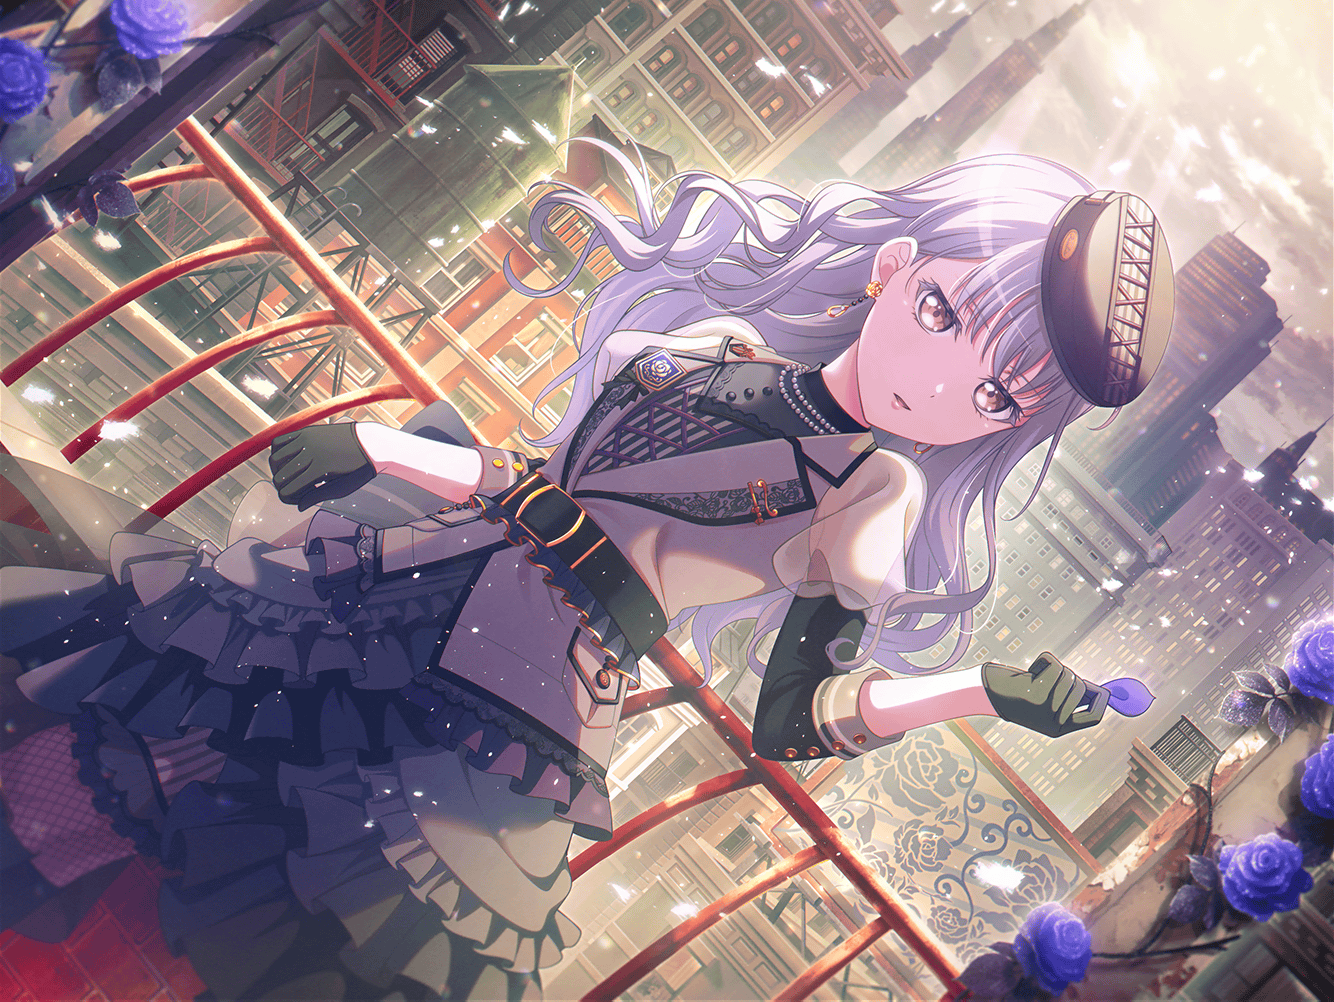
\includegraphics[width=1\linewidth]{fig.png}
    \caption{图片标题}
    \label{fig:关于如何使用LaTeX编写模板-标签}
\end{figure}

\begin{attention}
    在引用图片时,务必使用\verb|\ref{fig:节标题-标签}|进行引用。例如,图\ref{fig:关于如何使用LaTeX编写模板-标签}。不要使用“如上图”、“如下图”的表述形式,以免图片位置发生移动造成指代不明。
\end{attention}

\subsection{代码}\label{subsec:关于如何使用LaTeX编写模板-代码}

代码使用\verb|lstlisting|环境。

\begin{lstlisting}
SYSTEM = O
ISMEAR = 0
SIGMA = 0.05
NSW = 1
\end{lstlisting}

如果希望在代码左侧添加行号以示说明,请在引用环境的右侧添加\verb|numbers=left|设置,即采用下面的代码:

\begin{lstlisting}[frame=line]
\begin{lstlisting}[numbers=left]
    ..
\end{lstlisting}

得到效果如下所示

\begin{lstlisting}[numbers=left]
SYSTEM = O
ISMEAR = 0
SIGMA = 0.05
NSW = 1
\end{lstlisting}

\begin{attention}
    若你希望在代码块中添加代码名称(例如文件名),可以使用\verb|caption|选项进行说明,例如,下面的代码:
    \begin{lstlisting}[frame=line]
\begin{lstlisting}[caption=简单的INCAR文件]
    ..        
    \end{lstlisting}

    实际编译后结果为
    \begin{lstlisting}[caption=简单的INCAR文件]
SYSTEM = O
ISMEAR = 0
SIGMA = 0.05
NSW = 1
    \end{lstlisting}

\end{attention}

\subsection{添加索引}\label{subsec:关于如何使用LaTeX编写模板-添加索引}

建议在编写过程中,为文中的程序关键字创建索引。为方便使用,可以使用命令\verb|\keyword{}|。例如,在VASP讲解SIGMA函数时,可以使用下面的代码

\begin{lstlisting}[frame=line]
\keyword{SIGMA}
\end{lstlisting}

从而在表述关键字的同时创建索引。同时,也可以使用\verb|\keywordin{}{}|的形式创建带有所属关系的索引,例如

\begin{lstlisting}[frame=line]
\keywordin{INCAR}{SIGMA}
\end{lstlisting}

便是创建了属于\code{INCAR}条目下的\code{SIGMA}索引。

\begin{attention}
    在编写时,鼓励使用索引方便他人根据关键字直接检索。在创建索引时,请提前确认现有的索引表是否有现成的索引。例如,\\\verb|\keyword{SIGMA}|和\verb|\keywordin{INCAR}{SIGMA}|会得到不同的结果。

    同时,在编写过程中已经将输出和索引集成在一个命令中,你不需要特地再编写一个输出的命令如\code{SIGMA$\backslash$keyword\{SIGMA\}},只需要使用\\\code{$\backslash$keyword\{SIGMA\}}便可在输出\code{SIGMA}的同时创建索引。
\end{attention}

对于一些特殊的内容,可能不希望给出索引(通常是命令或者文件名等),它们既不属于关键字,也不属于简单的英文单词。为了将它们区分,使用\verb|\code{}|命令进行编写。例如,\verb|\code{cd \$OLDPWD}|的输出结果为\code{cd \$OLDPWD}

\begin{attention}
    在一些特殊的情况下(例如上面的例子),可能会包含\LaTeX 本身的特殊符号(如\$本身作为公式符号)。在输入时,应当使用反斜杠$\backslash$ 作为转义字符。
\end{attention}


    \mainmatter

    \part{Linux基础}

    \chapter{Linux命令行操作}\label{chap:Linux命令行操作}
\minitoc
% 请在下方的大括号相应位置填写正确的节标题和标签,以及作者姓名
\section{认识Linux目录}\label{sec:认识Linux目录}
\sectionAuthor{Jiaqi Z.}

% 请在下方的item内填写本节知识点
\begin{Abstract}
    \item Linux命令格式
    \item 如何在Linux当中表示目录
    \item 绝对路径和相对路径
    \item 如何快速表示当前目录和上一级目录
\end{Abstract}

% 请在正文相应位置填写正确的小节标题(或小小节标题),同时将标签的“节标题”和“小节标题”改为实际内容

\subsection{命令格式}\label{subsec:认识Linux目录-命令格式}

与Windows使用可视化界面不同,Linux大多时候使用命令行(shell)进行操作。因此,在Linux的学习过程中,一个最重要的任务,就是掌握一些常见的Linux命令。对于大多数科研课题组而言,Linux系统都是在远程云端服务器上,因此在本地往往只需要一个终端程序即可连接到服务器。一些常见的终端软件包括Xshell、MobaXterm、甚至VS Code\footnote{对于VS Code而言,可能需要扩展插件(例如Remote-SSH)的支持}等。

\begin{attention}
    如果你熟悉其他操作系统,可能听闻过类似于Windows Server,或者Linux的Ubuntu这样的操作系统。明明也可以使用可视化界面,为什么在科研过程中从来不会用到它们呢?(更严谨地说,在远程服务器上)。实际上,当使用可视化界面进行远程连接时,所产生的网络资源消耗是巨大的,通常需要更大的带宽,而使用命令行就可以提高数据传输效率。此外,更重要的一点是,使用命令行可以很容易实现批量处理,这在后续的章节会介绍到。
\end{attention}

在Linux当中,输入命令通常采用的格式是\code{命令 [-选项] [参数]},其中中括号表示这个部分是\emph{可选的},即可以没有的。例如,当我们希望列出当前目录下所有文件时,可以使用\keyword{ls}直接输出,也可以使用\code{ls -l}以列表格式输出。

\begin{attention}
    在后面可能会看到选项有多个的情况,此时为了简化,可以将选项合并在一起。例如,\code{ls -l -a}可以简化为\code{ls -la}。

    命令与选项、参数之间是以空格进行分割,且这个空格不能省略。
\end{attention}

\subsection{目录表示方法}\label{subsec:认识Linux目录-目录表示方法}

在Linux当中,所有目录都是以根目录\code{/}为起点,任何目录都是根目录的子目录。根目录下存在一些固定的目录(这些目录通常有特定的含义),例如,在根目录下有一个叫做\code{bin}的目录(通常写作\code{/bin}),它存放的都是\emph{二进制文件},也就是系统可以执行的程序文件。

\begin{attention}
    在Linux当中,任何命令实际上都是可执行程序。你可以在\code{/bin}目录下看到后面所学的所有Linux终端命令。
\end{attention}

另一个比较重要的位置是家目录\code{/home},它存放的是用户个人文件。在这一目录下,你可以看到系统所注册的所有用户名。但是,这些文件夹大多数是无法查看的\footnote{这涉及到Linux操作权限的问题,通常来说,权限分为三组,即所有者权限、所属组权限和其他用户权限。对于\code{/home}目录下而言,所有目录都是对所有者(即这个用户本身)提供全部权限,而其他人无法访问、修改。}。对于用户自己的家目录,通常也可以表示为\code{\~}。通常来说,当你使用终端等连接登录时,默认的所在目录就是家目录\code{\~}

\subsection{绝对路径和相对路径}\label{subsec:认识Linux目录-绝对路径和相对路径}

任何目录在操作时都具有两种表示方式,\emph{绝对路径}和\emph{相对路径}。正如\ref{subsec:认识Linux目录-目录表示方法}所介绍的那样,任何目录都是从根目录开始的。因此在描述一个目录时,可以从根目录(即\code{/})开始。例如,若你在你的家目录下有一个叫做\code{vasp}的目录,那么它的绝对路径就是\code{/home/<你的用户名>/vasp}。

随着层级逐渐增多,这种表示方法也会越来越复杂,因此,在表示一个目录时,默认也可以从当前所在目录开始算起(即\emph{相对路径})。例如,若你刚刚进入终端,此时所在目录就是\code{\~}目录,即\code{/home/<你的用户名>}下,此时若想表示\code{vasp},则只需要使用\code{vasp}即可。

\begin{attention}
    在这种情况下,你可以将目录\code{vasp}理解为\code{<当前所在目录>/vasp},即等价于\code{/home/<你的用户名>/vasp}。

    千万不要写成\code{/vasp},它表示根目录下的\code{vasp}目录。如果你希望特别强调当前目录,可以使用符号\code{.}(一个点)表示“当前目录”,即可以写成\code{./vasp}
\end{attention}

然而,在这种情况下,回到\emph{当前目录的上一级目录}是麻烦的,即在目前所学范围内,只能使用绝对路径。好在Linux提供了一个命令:\code{..}(两个点)表示\emph{上一级目录}。因此,如果你当前处在目录\code{/home/<你的用户名>/vasp}当中,则\code{..}表示\code{/home/<你的用户名>}

同理,\code{../..}表示父目录的父目录,在上面的例子中即为\code{/home}目录。

\begin{attention}
    在终端当中,\code{..}(两个点)表示父目录(即上一级目录),而一个点\code{.}表示当前目录。

    这些符号(指令)在后续关于目录操作中都是可以使用的。
\end{attention}

看到这里,可以思考下面的问题:如果在你的家目录下有两个目录\code{python}和\code{vasp},此时你在\code{/home/<你的用户名>/vasp}目录下,如何可以快速表示\code{python}目录呢(不能使用绝对路径)?答案在下面

答案:\rotatebox{180}{\code{../python}即可表示\code{/home/<你的用户名>/python}目录}
% 请在下方的大括号相应位置填写正确的节标题和标签,以及作者姓名
\section{目录操作}\label{sec:目录操作}
\sectionAuthor{Jiaqi Z.}

% 请在下方的item内填写本节知识点
\begin{Abstract}
    \item 如何显示当前目录下所有文件
    \item 如何创建目录
    \item 如何切换至其他目录
\end{Abstract}

% 请在正文相应位置填写正确的小节标题(或小小节标题),同时将标签的“节标题”和“小节标题”改为实际内容

\subsection{显示目录文件\keyword{ls}}\label{subsec:目录操作-显示目录文件}

在这一节以及下一节,我们将讨论如何对目录和文件做基本的操作。无论是哪一种,一个最基本的前提是\emph{知道当前目录有哪些文件和目录},从而才能进行后续操作(例如编辑、删除、移动、进入目录等)

在Linux当中,列出一个目录下所有文件使用的是\code{ls}命令。在没有任何参数与选项的前提下,它输出的结果就是\emph{当前所在目录下的所有文件和目录}。以\ref{subsec:认识Linux目录-绝对路径和相对路径}一节最后的例子为例,家目录下有\code{vasp}和\code{python}两个目录,当在家目录下执行\code{ls}命令时,结果如下:

\begin{lstlisting}[language=bash]
$ ls
vasp  python
\end{lstlisting}

同时,\code{ls}支持在后面添加一个参数表示要输出的目录。例如,在这一例子下,若在家目录当中执行命令\code{ls vasp},将会输出\code{vasp}目录下的所有文件和目录。利用\code{..}表示上一级目录的用法,若当前处在\code{\texttilde/vasp}目录下,使用\code{ls ..}便可得到上一级目录(即家目录)下的所有文件和目录。

\subsubsection{\keywordin{ls}{ls -l}}

下面介绍两个常见的\code{ls}选项,首先是\code{-l}选项,它表示\emph{以列表形式输出结果}。例如,还是上面的例子,使用这一命令的结果为:

\begin{lstlisting}[language=bash]
$ ls -l
total 0
drwxrwxr-x 2 zjq zjq 6 Aug 12 16:35 python
drwxrwxr-x 2 zjq zjq 6 Aug 12 16:35 vasp
\end{lstlisting}

\begin{extend}
每一个文件的输出结果可以分为9个部分,分别是:权限、文件硬链接数或目录子目录数、拥有者用户名、拥有者所在组、文件大小、文件修改月份、日期、时间、文件名。

关于权限,可以将其分成四部分:第一部分(一个字符)表示文件类型(这里的d表示目录),第二部分(三个字符)表示拥有者权限(rwx表示可读可写可执行),第三部分(三个字符)表示组用户权限,第四部分(三个字符)表示其他用户权限(r-x)表示可读,可执行但不可编辑。

对于文件硬链接数和目标子目录数,对于初始创建的文件而言,通常为1,而对于目录而言,默认为2(因为有两个子目录\code{.}和\code{..})
\end{extend}

有时,也可以使用\keyword{ll}代替指令\code{ls -l},其二者是完全等价的。

\subsubsection{\keywordin{ls}{ls -a}}

\code{-a}选项表示\emph{列出所有文件,包括隐藏文件}。例如,在\code{\texttilde/vasp}目录下,使用\code{ls -a}命令,结果为:

\begin{lstlisting}[language=bash]
$ ls -a
.  ..
\end{lstlisting}

\begin{extend}
    正如前面所介绍的那样,任何一个空目录都会默认有两个隐藏目录--自身和它的上一级目录。而这也解释了\ref{subsec:认识Linux目录-绝对路径和相对路径}一节所介绍的\code{.}和\code{..}的本质,它们实际上就是任何当前目录下的两个子目录。
\end{extend}

\begin{attention}
    前面所介绍的\code{-l}选项和\code{-a}选项是可以合并使用的,此时可以将两个选项之间以空格分割,如\code{ls -l -a},或者将两个选项写在一起\code{ls -la}

    当选项写在一起时,选项的排列顺序不重要。

    与最开始介绍\code{ls}后面加参数表示目录一样,带有选项的\code{ls}同样可以在后面添加参数,例如,\code{ls -a vasp}表示列出当前目录下的\code{vasp}子目录下的所有文件和目录(包括隐藏文件)
\end{attention}

\subsection{关于隐藏文件}\label{subsec:目录操作-关于隐藏文件}

\begin{extend}
    隐藏文件是指在文件名前面加上\code{.}的,例如\code{.bashrc}。

    隐藏文件在Linux当中的常见用途有:
    \begin{itemize}
        \item 配置文件
        \item 临时文件
        \item 缓存文件
        \item 等
    \end{itemize}

    总而言之,隐藏文件是为了防止误操作而存在的。(这可能与一些人认为的“隐藏文件是避免别人看到”不同)事实上,哪怕在Windows操作系统中,隐藏文件也是存在且方便查看的\footnote{在Windows操作系统中,可以通过右键-属性-隐藏的方式将文件或文件夹设置为隐藏;相对地,对Windows10操作系统而言,可以通过文件夹菜单栏的“查看”-“隐藏的项目”找到那些隐藏文件。只不过在Linux当中,隐藏文件使用前面加点\code{.}的方式设置,但无论如何,隐藏文件永远不是不让别人看见的方法,如果想达成这一目的,正确的方法是设置权限。}
\end{extend}

\subsection{创建目录\keyword{mkdir}}\label{subsec:目录操作-创建目录}

如果所有操作都在家目录下进行,那文件管理就太复杂了。试想一下,在科研里面算了好几年的结果,全部“一股脑”堆在一起,既难找,也容易忘记当时是做了什么。因此,一个好的目录管理至关重要。而前提,就是知道如何创建目录。

在Linux当中,创建目录的方法是使用\code{mkdir}命令。与前面介绍的\code{ls},以及后面要介绍的\code{cd}不同的是,\code{mkdir}必须带有一个参数,表示\emph{创建的目录路径}。对于刚开始接触的初学者,一个最简单的命令格式是:\code{mkdir <目录名>},其中表示在当前目录下创建一个名为\code{<目录名>}的目录。例如,希望在当前目录下创建一个名为\code{ML}的目录,则可以使用命令\code{mkdir ML}。

正如前面所介绍的路径,\code{mkdir}后面的路径也可以是绝对路径或相对路径。无论是哪种形式,其含义是一样的,即\emph{在你所描述的路径下创建目录}。利用这种方法,你可以在更远的层级关系下创建目录。例如,在\code{\texttilde/vasp/lattice/Fe}目录下创建\code{\texttilde/python/ML/plot}目录。

\begin{attention}
    你所写的路径名,应当是你所要创建的目录。这句话似乎有点绕,举个例子,如果你希望在\code{/home/zjq/vasp}下创建一个名为\code{lattice}的目录,则你需要运行的命令是\code{mkdir /home/zjq/vasp/lattice}。注意到,后面的路径实际上就是你要创建的目录。
\end{attention}

\subsection{切换目录\keyword{cd}}\label{subsec:目录操作-切换目录}

在Linux当中,切换目录使用的命令是\code{cd},通常来说,后面需要配合一个参数,表示\emph{要切换到哪里}。例如,使用命令\code{cd /home}则是将当前目录切换到\code{/home}目录下。配合以\code{..},可以使用\code{cd ..}切换到上一级目录。

思考:如果使用\code{cd .},会得到什么结果?

\answer{这个命令的含义是\emph{切换到当前目录},最终效果就是什么也不发生}

特殊的,对于家目录而言,除了可以使用\code{cd \texttilde}外,Linux也支持直接使用\code{cd},不添加任何参数实现这一功能,即二者是等价的。

\subsection{错误处理}\label{subsec:目录操作-错误处理}
% 请在本节列出可能遇见的错误与解决方法

\subsubsection{-bash: cd: <目录名>: Not a directory}

\code{cd}后面的参数必须是目录,不能是文件。如果参数是文件,则会报该错误。

如果不知道哪个是目录,哪个是文件,可以使用\code{ls -l}查看第一个字符(文件类型),如果第一个字符是\code{d},则表示目录,如果是\code{-},则表示文件\footnote{在一些比较新的终端程序中,可能会将文件和目录以不同颜色区分。例如,在MobaXterm当中,默认情况下文件是白色,目录是蓝色。当然,这些颜色设置都是可以通过Settings-Terminal-Default color settings设置颜色主题,这里所说的这一例子为“Dark background / Light text”主题}。例如,

\begin{lstlisting}[language=bash]
$ ls -l
total 4
-rw-rw-r-- 1 zjq zjq 4 Aug 12 17:12 INCAR
drwxrwxr-x 2 zjq zjq 6 Aug 12 16:35 python
drwxrwxr-x 2 zjq zjq 6 Aug 12 16:35 vasp
\end{lstlisting}

表示\code{INCAR}是文件,而\code{vasp}和\code{python}是目录。如果执行了\code{cd INCAR},则会报错。

\subsubsection{-bash: cd: <目录名>: Permission denied}

这表明你尝试进入一个你没有权限的目录。例如,在\code{/home}目录下,有\code{ljk}和\code{zjq}两个目录,分别表示两个用户。如果执行\code{ls -l}则会发现:

\begin{lstlisting}[language=bash]
$ ls -l
total 32
drwx------  13 ljk    ljk    4096 Aug  5 17:34 ljk
drwx------  75 zjq    zjq    4096 Aug 12 17:12 zjq
\end{lstlisting}

很显然,每个目录只有目录拥有者自己可以访问。例如,作为用户\code{zjq},当尝试执行\code{cd ljk}时,则会报错。

\begin{extend}
    这种情况有一个特例:root用户。对于root用户而言,可以进入任何目录。但通常来说,root用户是由服务器管理者所持有的,作为一般用户而言,不需要也不应该进入没有权限的目录,或者执行没有权限的操作\footnote{“删库跑路”这件事对于一般用户来说是不可能的}。
\end{extend}

\subsubsection{mkdir: cannot create directory <目录名>: No such file or directory}

虽然我们说可以用绝对路径或相对路径在更远的层级关系下创建目录。但这一操作的前提是,\emph{这个目录的上一级目录需要存在}。例如,当你执行\code{mkdir vasp/lattice/Fe}时,首先需要确保目录\code{vasp}和\code{vasp/lattice}存在,才会创建\code{vasp/lattice/Fe}。如果你要创建的目录其上一级目录不存在,则会报错。

一个很自然的解决方法是:\emph{一层一层创建}。这种方法虽然麻烦,但可以确保目录是清晰的\footnote{如果你确实想要一个快捷的方法,可以使用选项\code{-p}。这一选项可以在遇到没有的目录时自动为你创建。例如,上面的例子也可以直接使用\code{mkdir -p vasp/lattice/Fe},但这一操作需要保证输入内容是正确的。一旦有内容输错,则极有可能造成目录结构混乱。}。

\subsubsection{mkdir: missing operand}

很显然,你在使用\code{mkdir}时没有给任何参数。正如\ref{subsec:目录操作-创建目录}所说的那样,在调用\code{mkdir}时\emph{必须提供一个参数表示要创建的目录路径}。
% 请在下方的大括号相应位置填写正确的节标题和标签,以及作者姓名
\section{文件操作}\label{sec:文件操作}
\sectionAuthor{Jiaqi Z.}

% 请在下方的item内填写本节知识点
\begin{Abstract}
    \item 如何移动文件(目录),如何给文件(目录)重命名
    \item 如何删除文件(目录)
    \item 如何复制文件(目录)
\end{Abstract}

% 请在正文相应位置填写正确的小节标题(或小小节标题),同时将标签的“节标题”和“小节标题”改为实际内容

这一节,我们专注于文件的相关操作。类似于Windows的基本操作,Linux的文件操作也无外乎就是\emph{移动、删除、复制}。同时,这一节的许多命令对于文件和目录都是适用的,但可能会有一个注意事项,这往往会出错。

\subsection{移动文件\keyword{mv}}\label{subsec:文件操作-移动文件}

在Linux当中,移动文件使用的命令是\code{mv}。其基本用法是\code{mv <源文件路径> <目标文件路径>}。例如,我们在\code{vasp}目录下,希望将里面的\code{OUTCAR}移动至上一级目录,可以使用\code{mv OUTCAR ..}。类似地,对于更复杂的文件移动,只不过在描述路径时稍微复杂一点,其他的步骤没有什么不同。

如果你足够敏感,也许会发现一点问题:\emph{为什么前面的命令,\code{OUTCAR}是文件,而\code{..}是目录}?两个难道不应该统一吗?

对于这个问题,可以分两个部分讨论:如果前面是文件,后面也是文件,例如\code{mv OUTCAR ../OUTCAR},这个命令与前面的命令效果是完全等价的。但是,有趣的地方在于,如果你试着执行\code{mv OUTCAR ../INCAR}的话,你会发现,Linux将\code{OUTCAR}移动到\code{..}的同时,还将其改名为\code{INCAR}。

进一步想一下,如果我们现在直接写成\code{mv OUTCAR INCAR}的话,可以将其看作把当前目录下的\code{OUTCAR}移动至当前目录,同时改名为\code{INCAR},总的效果就是,文件被重命名为\code{INCAR}。

\begin{attention}
    正如你所见到的那样,Linux没有单独的重命名文件命令,而是通过\code{mv}命令来完成。
\end{attention}

进一步,如果前后两个参数都是目录会发生什么呢?很简单,\emph{就是将前面的目录移动至后面的目录},从效果上看,近似于将第一个参数的目录看作文件。

\begin{attention}
    与文件移动类似的操作,如重命名,对目录的移动同样成立。
\end{attention}

\subsection{如何删除文件\keyword{rm}}\label{subsec:文件操作-如何删除文件}

相比于移动文件需要两个参数,删除文件的命令\code{rm}只需要一个参数即可,也许你也能猜到这个参数的含义,即\code{rm <删除的文件路径>}。例如,要删除当前目录下的\code{INCAR}文件,只需要执行\code{rm INCAR}即可。同样的,你也可以使用更复杂的绝对路径或相对路径,例如,删除上一级目录下的\code{OUTCAR}文件,可以使用\code{rm ../OUTCAR}。

\begin{extend}
    与Windows不同,Linux删除文件通常是直接删除,而不是放在所谓的\emph{回收站}内。因此,在删除文件时务必小心。

    在有些版本的Linux(例如Ubuntu)当中,删除的文件被移动至\code{/home/<用户名>/.local/share/Trash/files}当中,这个目录起到的临时的\emph{回收站}功能,但你不应该寄希望于这个功能,而是仔细检查删除文件的正确性,并做好合适的备份。
\end{extend}

对于删除目录而言,情况有点特殊,需要使用\keywordin{rm}{rm -r}命令删除一个目录,此时后面所接参数为目录的路径,例如,删除当前目录下的\code{vasp}目录,则可以使用\code{rm -r vasp}。

\begin{attention}
    \code{-r}选项通常表示\emph{递归},例如,在\code{rm -r}当中,表示\emph{递归删除},从而达到删除一个目录的效果。在删除目录时会连同里面的所有内容都删除掉,因此需要特别小心。

    如果担心删除错误的文件,可以在选项中使用\code{-i}。\keywordin{rm}{rm -i}表示\emph{在删除时}询问是否删除。

    对于空目录而言,Linux还提供了一个命令\keyword{rmdir},其用法为\code{rmdir <目录路径名>},可以删除一个\emph{空目录}。
\end{attention}

\subsection{如何复制文件\keyword{cp}}\label{subsec:文件操作-如何复制文件}

复制文件的命令为\code{cp},其用法与移动文件\code{mv}几乎完全一样,无非就是将\emph{移动}改为\emph{复制}。简单来说,语法就是\code{cp <源文件路径> <目标文件路径>},类似于\ref{subsec:文件操作-移动文件}当中所介绍的重命名方法,使用\code{cp}命令同样可以做到复制的同时重命名。例如,\code{cp vasp/OUTCAR ../INCAR}表示将\code{vasp}目录下的\code{OUTCAR}文件复制到上一层目录,并重命名为\code{INCAR}

如果想要复制一个目录,也需要使用选项\keywordin{cp}{cp -r}。例如,\code{cp -r vasp/ python/}表示将\code{vasp}目录复制到当前目录并重命名为\code{python}。

\begin{attention}
    我们在上面的命令当中使用\code{vasp/}和\code{python/}表示两个目录。其中使用了符号\code{/}作为结尾,这个符号通常强调该路径是个目录。对于Linux本身而言,有没有这个符号并没有区别。例如,\code{cp -r vasp python}也可以表示上面的操作。我们这么写只是为了强调这两个路径是目录而不是文件。
\end{attention}

\subsection{一次性处理多个文件}\label{subsec:文件操作-一次性处理多个文件}

前面介绍的\code{rm},\code{cp},\code{mv},以及在\ref{sec:目录操作}一节所介绍的\code{mkdir},都是可以针对多个文件同时操作的。以\code{rm}为例,如果想同时删除多个文件,只需要在后面添加多个参数即可,其中参数之间以空格分割。例如,\code{rm INCAR KPOINTS}表示删除当前目录下的\code{INCAR}文件和\code{KPOINTS}文件。对于\code{mkdir}创建多个目录而言,也是一样的用法,例如,使用\code{mkdir vasp ML}表示在当前目录下创建\code{vasp}目录和\code{ML}目录。

对于\code{cp}和\code{mv}而言,情况稍有不同。它们自身就需要两个参数,第一个是源路径,第二个是目标路径。如果有多个文件需要处理,Linux默认\emph{最后一个路径为目标路径,前面的所有参数都是源路径}。例如,\code{cp INCAR KPOINTS POSCAR POTCAR ..}表示将\code{INCAR},\code{KPOINTS},\code{POSCAR}和\code{POTCAR}复制到上一级目录中。

\begin{attention}
    对于\code{cp}和\code{mv}而言,若一次性移动多个文件,则最后一个参数必须是目录。这就意味着不能进行重命名操作。
\end{attention}


\subsection{错误处理}\label{subsec:文件操作-错误处理}
% 请在本节列出可能遇见的错误与解决方法

\subsubsection{rmdir: failed to remove <路径名>: Directory not empty}

使用\code{rmdir}命令时,\emph{只能用来删除空目录}。当要删除的目录不是空目录时,执行该命令则会报错。使用\code{rm -r <路径名>}往往是删除非空目录的常见方法。

\subsubsection{cp: -r not specified; omitting directory <路径名>}

当使用\code{cp}复制目录时,需要添加\code{-r}选项。如果没有添加这一选项则会报错。

\subsubsection{cp: target <路径名> is not a directory}

这通常出现在尝试使用\code{cp}复制多个文件时,最后的参数\emph{必须是目录}。如果此时不是目录,则会报错。

\subsubsection{rm: cannot remove <路径名>: Is a directory}

类似于\code{cp}复制目录,使用\code{rm}删除目录时,也需要添加\code{-r}选项。特别地,对于一次性删除多个文件,如果在删除文件的同时也存在把目录删除的情况,也需要添加这一选项。

\subsubsection{rm: remove write-protected regular file <文件名>? }

当你尝试对没有权限(不可写)的文件进行删除时,会提示该错误。关于权限的内容,将在\ref{sec:文件权限管理}一节详细讨论。在Linux当中,是有方法对文件权限进行修改的,但这并不是一个明智的方法。仔细检查文件操作,遵守这些权限,不要“越界”,可以保证你“安全”地使用操作系统(不会引起系统崩溃等严重问题)。

如果你确实需要删除,则只需要输入\code{y}(表示“yes”)并回车即可;反之则输入\code{n}(表示“no”)。


% 请在下方的大括号相应位置填写正确的节标题和标签,以及作者姓名
\section{查看文件}\label{sec:查看文件}
\sectionAuthor{Jiaqi Z.}

% 请在下方的item内填写本节知识点
\begin{Abstract}
    \item Linux文件类型
    \item 如何查看Linux文件
\end{Abstract}

% 请在正文相应位置填写正确的小节标题(或小小节标题),同时将标签的“节标题”和“小节标题”改为实际内容

这一节看似知识点不多,但命令还是挺多的。因此,一节只讲这一部分内容完全足够了。

\subsection{Linux文件类型}\label{subsec:查看文件-Linux文件类型}

\begin{extend}
    在\ref{subsec:目录操作-显示目录文件}当中,我们介绍了\code{ls -l}命令可以以列表形式查看文件。当时仅仅提到,第一个字符如果是\code{d}则表示\emph{目录},如果是\code{-}则表示\emph{普通文件}。在这一部分,我们稍微详细介绍一下更多的文件类型。

    \begin{itemize}
        \item 普通文件(\code{-}):就是普通的文件,通常可以分为\emph{文本文件},\emph{可执行文件}和\emph{压缩文件}等;
        \item 目录(\code{d}):在Linux当中,目录也是一种文件,该文件下存放的是这一目录下的\emph{inode}号(又名\emph{索引节点})和文件名等信息。当执行打开文件时,Linux实际上是通过inode号找到当前文件所在block(8个磁盘扇区组成一个block),从而执行文件;
        \item 设备文件,又分为\emph{块设备文件}(\code{b})和\emph{字符设备文件}(\code{c})。其中前者可以以“块”为单位进行访问(例如硬盘,软盘等),而后者则是以“字节流”的方式访问(例如字符终端、键盘等)。一般来说,设备文件存放在\code{/dev/}目录下;
        \item 链接文件(\code{l}):一般情况下指的是符号链接(软链接),类似于Windows操作系统下的“快捷方式”。创建符号链接的方法是使用\keyword{ln}的\keywordin{ln}{ln -s}选项\footnote{相对地还有“硬链接”,直接使用\code{ln}即可。对于硬链接而言,二者本质上是一个文件(类似于做了备份),当其中一个删除时,另一个不会删除;当其中一个文件修改时,另一个也会同时修改},例如,\code{ln -s INCAR INCAR\_link}表示创建了一个指向\code{INCAR}文件的链接文件\code{INCAR\_link}。当源文件删除时,符号链接文件也会删除;
        \item 管道文件(\code{p}):通常用于进程间的通信,创建方法是\keyword{mkfifo}命令\footnote{也许你会疑惑为什么是fifo而不是管道的单词pipe。事实上,FIFO是一种数据缓存器执行方法,即“先进先出”(First In First Out)。作为数据缓存器,其与普通存储器的区别是没有外部读写地址线,这样使用起来非常简单,但缺点就是只能顺序写入数据,顺序的读出数据。数据地址在内部由指针自动加1实现,而不能通过地址线寻找地址。而Linux进程间的通信大多就是采用这种通信方式,这种方式也是管道的特性。相对的,还有一种LIFO,即“后进先出”(Last In First Out),通常“堆栈”(Stack)就是采用这种方法。},即\code{mkfifo fifo\_file}。
        \item 套接字文件(\code{s}):用于通信(尤其是网络上的通信)。简单来说,这是为了避免多个进程或多个TCP连接同时在一个TCP协议端口传输数据造成混淆。一般来说,套接字文件包含目的IP地址,传输层使用协议(TCP或UDP)和使用的端口号,利用套接字文件将三个参数组合起来,从而在传输过程中实现并发服务。
    \end{itemize}
\end{extend}

\subsection{查看文件内容\keyword{cat},\keyword{tac}}\label{subsec:查看文件-查看文件内容}

在整个Linux使用过程中,最关键的仍然是\emph{普通文件}和\emph{目录}。虽然其他文件对于操作系统本身而言也很重要,但对于非计算机相关专业的科研用户而言,其意义不大。上面的介绍仅仅是作为一个补充。下面地内容将专注在文件本身。首先一个关键的问题是:\emph{如何查看文件内容}。

\begin{attention}
    当然,从文件操作本身来说,第一件事应当是创建文件。但是,创建文件需要的内容较多(例如,需要一些\code{vi}编辑器的使用,可能还需要重定向命令,在后面的章节再详细介绍。
    
    如果是初学者,希望可以尽快上手的话,你可以试着在Windows本地用记事本创建一个文本文件,并在里面随意输入一些你喜欢的文字(建议使用英文,对于中文等非ASCII字符而言,可能会出现乱码。),然后利用远程终端将文件发送至服务器(对于MobaXterm而言,在终端左侧有一个目录列表,你可以直接将文件拖拽至相应的目录中;对于其他终端软件,请参考其软件具体的操作方法)。后面对文件的查看操作,都可以对这个文本文件进行。
\end{attention}

首先需要了解的是,如何查看完整的文件。在Linux当中,查看文件内容的命令是\code{cat},其基本用法是\code{cat <文件路径名>}例如,对于位于当前目录下的\code{INCAR}文件,可以使用\code{cat INCAR}查看其内容。

\code{cat}命令有一些常用选项,例如,可以使用\keywordin{cat}{cat -n}或\keywordin{cat}{cat -b}显示行号,二者的区别在于前者会显示所有行号,而后者只对有内容的行显示行号。如果文本中空行内容太多,可以使用\keywordin{cat}{cat -s}对空行进行压缩,使其缩减为一个空行。

相对地,命令\code{tac}也是查看所有内容,只不过它是\code{从最后一行倒着输出}。可以看出,\code{tac}本身就是命令\code{cat}倒着写。例如,\code{tac INCAR}表示从最后一行开始输出\code{INCAR}文件。

\begin{attention}
    命令\code{cat}并不是单词“猫”的意思,而是连接concatenate的缩写。正如单词所表示的那样,\code{cat}最原始的功能,是连接多个文件。例如,有一个文件叫\code{a},另一个文件叫\code{b},执行命令\code{cat a b},则会将两个文件内容按照顺序连接起来并输出。
\end{attention}

\subsection{关于文件后缀名}\label{subsec:查看文件-关于文件后缀名}

对于熟悉Windows的用户而言,看到上面(包括之前的所有示例)也许都会有一个疑惑:在Linux当中,文件名为什么没有后缀?事实上,后缀名的重要性仅仅是Windows操作系统给你的一个“错觉”,让你误以为\emph{后缀名很重要}。事实上,\emph{Windows操作系统的文件名后缀并不会影响这个文件本身}。

例如,在Windows操作系统下创建一个文本文件,后缀名为\code{.txt},此时试着将其后缀名改为\code{*.mp3}或者\code{*.jpg}等,并再次在打开方式中用记事本打开(如果使用默认的打开方式一定会出现错误,例如音乐播放器或者图片查看器等)。可以发现,用记事本打开的结果与之前的文本文件内容是完全一样的。

\begin{attention}
    虽然表示后缀名的\code{.}可以任意放置,但有一个地方比较特殊--文件名开头。对于以\code{.}开头的文件名而言,它表示的含义是隐藏文件(这在\ref{subsec:目录操作-关于隐藏文件}一节介绍过了)
\end{attention}

对于Windows操作系统而言,使用后缀名往往是为了决定文件的打开方式(取决于Windows特有的\emph{注册表});而Linux文件大多都是文本文件(甚至系统配置也是文本文件),因此在Linux当中,文件后缀名就变得不重要了。也正因如此,在Linux当中你可以类似于Windows后缀名的方式创建任何的后缀(\code{*.jpg},\code{*.xyz}甚至\code{*.zjq},\code{*.ykn}都是可以的),在Linux看来,它们仅仅是文件名的一部分。

甚至,在Linux当中,大多时候文件都是没有后缀名的。这也就是之前的\code{INCAR}和\code{OUTCAR}为什么没有后缀。对于从Windows创建的文本文件上传至服务器而言,可能还留有所谓的后缀名\code{*.txt},你完全可以使用\code{mv}命令将后缀名删去,丝毫不影响文件本身和其他命令的运行。

\subsection{按页查看文件\keyword{more},\keyword{less}}\label{subsec:查看文件-按页查看文件}

使用\code{cat}和\code{tac}查看文件,都是“一股脑”输出到终端里,对于比较短的文件而言,这种方法是可行的;如果这个文件很长,则要上下翻页就会比较繁杂。

对于多页的文件而言,Linux可以使用\code{more}命令查看。基本用法是\code{more <文件路径名>}。例如,使用\code{more ../band/OUTCAR}就可以查看上一级目录下的\code{band}目录下的\code{OUTCAR}文件。在查看过程中,可以\emph{使用空格进行翻页,使用回车进行下一行查看}。

在查看过程中,可以随时使用\code{q}键退出。

对于一些需要往回翻页查看的文件,可以使用\code{less}命令。基本调用格式与\code{more}类似,即\code{less <文件路径名>}。与\code{more}不同的是,\code{less}命令可以向上翻页(使用\code{Page Up}键或者\code{b}键)\footnote{除次之外,也可以使用\code{d}向后翻半页,使用\code{u}向前翻半页。}

\begin{attention}
    对于\code{more}而言,实际上也可以通过\code{b}键实现向前翻一页的效果。但相比于\code{less}而言,\code{more}的自由性并不是太高。而且,使用\code{b}向前翻页的效果对于管道文件无法实现。

    此外,\code{less}还有更复杂的“搜索功能”,例如,可以使用符号\code{/<字符串>}的方法实现向下搜索,使用符号\code{?<字符串>}的方法实现向上搜索。同时,\code{less}的其他命令都是在显示文件后的操作,并不是类似于之前的“选项”(即使用\code{-}的形式),这种方法与vi的使用类似。
\end{attention}

无论是\code{more}还是\code{less},都可以使用\code{q}键退出显示文件。

\subsection{取头部\keyword{head}和取尾部\keyword{tail}}\label{subsec:查看文件-取头部和取尾部}

有时,可能会希望仅仅查看一个文件的开头或者结尾。此时可以使用Linux操作系统下的\code{head}和\code{tail}命令。这两个命令的基本调用方法都是一样的,即\code{head <文件路径名>}和\code{tail <文件路径名>}。例如,使用\code{head POSCAR}就可以查看当前目录下\code{POSCAR}文件开头几行,同理,使用\code{tail relax/OSZICAR}就可以查看\code{relax}目录下的\code{OSZICAR}文件结尾几行。

\begin{attention}
    通常情况下,直接调用\code{head}和\code{tail}得到的都是开头(或结尾)10行的内容。在有些时候,可能会希望输出更多行,或者少输出几行避免混乱。此时可以使用参数\keywordin{head}{head -n}和\keywordin{tail}{tail -n}实现,其基本格式为\code{head -n <行数> <文件路径名>}和\code{tail -n <行数> <文件路径名>},这一选项表示输出指定的行数。例如,\code{head -n 5 POSCAR}可以查看\code{POSCAR}文件开头5行。对于\code{tail}同理。

    除此之外,\code{head}和\code{tail}还提供了选项\keywordin{head}{head -c}和\keywordin{tail}{tail -c},表示输出开头(或结尾)多少个字符的内容,格式与上面\code{-n}选项类似,即\code{head -c <字符数> <文件路径名>}和\code{tail -c <字符数> <文件路径名>}。
\end{attention}

\subsection{错误处理}\label{subsec:查看文件-错误处理}
% 请在本节列出可能遇见的错误与解决方法

\subsubsection{cat: <文件名>: Is a directory}

\code{cat}命令仅限于查看文件内容,若后面所接内容为一个目录,例如,\code{cat vasp/}则会报错

\subsubsection{输入\code{cat}命令后忘记输入文件名直接回车,输入文件名后结果只输出了文件名,并没有输出内容}

当直接调用\code{cat}而没有接任何参数时,表示将终端标准输入所读取到的内容输出到终端。对于普通调用\code{cat <文件路径名>}而言,是将读取到的文件输出到终端。若没有任何参数,则会读取后面输入的内容。

退出的方法则是使用\code{ctrl+d}键结束当前输入,或者使用\code{ctrl+c}键强制终止当前命令。

\subsubsection{cat: <文件名>: No such file or directory}

文件路径不存在,检查一下路径(尤其是当前工作路径)是否正确。

\subsubsection{head(或tail): invalid number of lines: <文件名>}

当你使用\code{head -n}或\code{tail -n}时,后面的行数是必须提供的一个参数。若没有提供行数,则会报错。

\subsubsection{head(或tail): cannot open <文件名> for reading: No such file or directory}

文件路径不存在,检查一下路径(尤其是当前工作路径)是否正确。

\subsubsection{head(或tail): error reading <文件名>: Is a directoryy}

类似于使用\code{cat}打开目录,使用\code{head}或\code{tail}打开目录就会报这种错误。

\subsubsection{使用\code{more}查看文件,输出*** <文件名>: directory ***}

这是因为试着用\code{more}查看目录而不是文件。

\subsubsection{使用\code{less}查看文件,输出许多奇怪的路径,不是想要的内容}

如果你仔细看一下里面的内容就会发现,当你用\code{less}查看目录时,输出的是这个目录下所有的文件和目录(包括隐藏文件)。事实上,使用\code{less <目录路径>}得到的结果和使用\code{ls -l <目录路径>}是一样的。只不过前者是单独输出的,而后者是直接输出在终端里。

\subsubsection{Missing filename ("less --help" for help)}

在调用\code{less}时忘记提供文件路径了。

\subsubsection{more: bad usage Try 'more --help' for more information.}

与上面的错误类似,在调用\code{more}时忘记提供文件路径了。
% 请在下方的大括号相应位置填写正确的节标题和标签,以及作者姓名
\section{压缩与解压缩}\label{sec:压缩与解压缩}
\sectionAuthor{Jiaqi Z.}

% 请在下方的item内填写本节知识点
\begin{Abstract}
    \item 如何压缩文件
    \item 如何解压缩文件
\end{Abstract}

% 请在正文相应位置填写正确的小节标题(或小小节标题),同时将标签的“节标题”和“小节标题”改为实际内容

\subsection{备份和压缩}\label{subsec:压缩与解压缩-备份和压缩}

\begin{extend}
    虽然在许多场合,会将Linux的一些使用\keyword{tar}的操作说成是压缩文件和解压缩文件,但这个表述实际上是不贴切的。事实上,\code{tar}的本意是tape archive,指的是“磁带存档”,是为将若干个文件归档到磁带上,从而方便备份而设计的。而压缩文件实际上在\code{tar}当中经历了另外的步骤,即gzip压缩,或者是bzip2压缩等。这些在命令上都是通过额外的选项实现的。

    但是,由于现在大多数时候都是习惯于将两个步骤合二为一,包括使用gzip压缩后得到的\code{.gz}文件也可以在Windows操作系统下解压缩,从而极大方便了文件之间的跨系统传输。因此,在通常情况下,我们使用到的都是“压缩”。这里之所以给出两者的不同仅作为补充扩展用,在后续表述中,往往不做区分,一律表述为“压缩”和“解压缩”。
\end{extend}

\subsection{使用\keyword{tar}命令压缩文件}\label{subsec:压缩与解压缩-使用tar命令压缩文件}

\code{tar}命令在使用时通常会配合许多选项,在官方文档中,选项就有50个左右甚至更多,因此,我们不可能在这里完全介绍完所有的选项。对于一般的科研工作而言,只需要掌握几个最基本的选项即可。

首先一个最基本的选项是\keywordin{tar}{tar -c},表示\emph{创建备份文件}。通常仅有这一个参数是不够的,还需要配合以如\keywordin{tar}{tar -f}参数,这一参数表示\emph{指定备份文件}。结合这两个选项,可以得到一个备份文件的基本模式为:\code{tar -cf <备份文件路径> <要备份的文件1路径> <要备份的文件2路径> ...}。例如,\code{tar -cf vasp.tar INCAR KPOINTS POSCAR POTCAR}表示将当前目录下的\code{INCAR},\code{KPOINTS},\code{POTCAR}和\code{POSCAR}备份至当前目录的\code{vasp.tar}当中。

\begin{attention}
    \code{-cf}后面的参数,除第一个是备份文件路径外,后面所有参数都是要备份的文件路径。
\end{attention}

正如\ref{subsec:压缩与解压缩-备份和压缩}所说的关于压缩和备份的区别一样,我们这里所做的仅仅是备份。对于真正的压缩,我们还需要添加一个压缩格式\footnote{所谓的\emph{压缩格式},在Windows系统下常见的如zip、rar等,而在Linux操作系统下,最常见的是gzip,当然也有如bzip、xz等。}。对于常见的gzip压缩格式而言,使用的选项是\keywordin{tar}{tar -z}。因此,一个完整的压缩命令可以表示为\code{tar -czf <压缩文件路径> <要压缩的文件1路径> <要压缩的文件2路径> ...}。

\begin{attention}
    一般情况下,使用gzip压缩的文件后缀名都是\code{.gz}。
\end{attention}

对于上面所提到的备份例子,你能想到它的压缩命令是什么吗?

\answer{\code{tar -czf vasp.tar.gz INCAR KPOINTS POSCAR POTCAR}}

\subsection{解压缩}\label{subsec:压缩与解压缩-解压缩}

相对地,有了压缩过程,就一定会有\emph{解压缩}过程。首先,先忽略掉压缩格式(即gzip等相关内容),仅仅从备份的角度,考虑它的逆过程,也就是\emph{还原文件}。

在\code{tar}当中,可以使用选项\keywordin{tar}{tar -x}实现备份文件的还原。例如,在开始的备份操作中,可以使用\code{tar -xf vasp.tar}实现对备份文件\code{vasp.tar}的还原。对于解压缩过程,选项完全类似,只需要使用\code{tar -xzf}即可。例如,对上面的\code{vasp.tar.gz}进行解压缩,可以使用\code{tar -xzf vasp.tar.gz}。

\subsection{查看压缩文件}\label{subsec:压缩与解压缩-查看压缩文件}

这里所说的查看压缩文件,主要指的是查看\emph{压缩包内的文件},从更广义的角度看,就是查看所谓的“备份”文件。

首先,在\code{tar}里面有一个选项\keywordin{tar}{tar -v},可以在压缩(解压)过程中查看压缩(解压)的文件。例如,上面的压缩和解压命令,分别可以写成\code{tar -cvf vasp.tar INCAR KPOINTS POSCAR POTCAR}和\code{tar -xvf vasp.tar}。对于gzip格式的压缩和解压缩,只需要在参数里额外添加\code{-z}即可。

另外一种可能的场景是已经存在一个压缩文件(例如\code{vasp.tar}),需要查看里面的内容。虽然直接解压查看是一种办法,但如果发现不是想要的文件再删除,就稍显麻烦(尤其是有多个文件时)。因此,Linux提供了一种类似于Windows直接查看压缩包文件的方法,即使用\keywordin{tar}{tar -t}表示列出压缩包内文件。

\begin{attention}
    在使用\code{tar -t}时,往往需要配合以\code{-f}参数指定压缩文件名。其完整用法为\code{tar -tf <压缩文件路径>}。例如,使用\code{tar -tf vasp.tar}可以查看\code{vasp.tar}压缩文件中的文件列表。

    无论是普通的备份文件,还是使用gzip压缩的文件,都是使用\code{tar -tf}查看(没有选项\code{-z})。

    使用\code{tar -tvf}同样可以得到文件列表,只是输出的内容更详细(类似于\code{ls -l}的输出结果)
\end{attention}

除此之外,查看压缩文件还有一种方法,使用\keyword{less}命令。通过\code{less <压缩文件路径>}可以直接查看压缩文件内容,其形式上类似于\code{tar -tvf}和\code{ls -l}。

\subsection{压缩文件的追加与合并}\label{subsec:压缩与解压缩-压缩文件的追加与合并}

虽然已经非常小心地创建了压缩文件,但有时还是会有遗漏。例如,当你将\code{INCAR},\code{POSCAR},\code{KPOINTS}和\code{POTCAR}已经添加到\code{vasp.tar}之后,突然发现还应当把\code{CONTCAR}添加进去。如果此时文件还保留着,当然,重新使用\code{tar -cf vasp.tar ...}也是可以的(其中...表示五个文件路径)。但是,如果之前的文件已经删除了呢?解压后再重新压缩也不是不可行,但总是麻烦一步。

在\code{tar}的选项中,提供了一个选项\keywordin{tar}{tar -r}表示\emph{将文件追加到压缩文件内}。例如,上面的例子,可以直接使用\code{tar -rf vasp.tar CONTCAR}即可将\code{CONTCAR}添加到\code{vasp.tar}中(哪怕原先的四个原始文件删除了也没关系)。

上面的例子是将文件追加到压缩文件内,如果是\emph{将压缩文件内的所有文件全部追加到另一个压缩文件里呢}?可以使用\keywordin{tar}{tar -A}选项。其格式为\code{tar -Af <追加的目标压缩文件路径> <追加的压缩文件路径>}。例如,我们已经有了包含\code{INCAR},\code{KPOINTS},\code{POSCAR},\code{POTCAR}的压缩文件\code{vasp.tar},此时又有一个压缩文件\code{result.tar},里面包含有\code{OUTCAR},\code{CONTCAR},如何将其合并到共同的\code{vasp.tar}当中呢?可以使用\code{tar -Af vasp.tar result.tar}。

\begin{attention}
    这里的选项\code{-A}是大写字母,千万不要写成小写字母。二者的含义不同,对于小写字母\keywordin{tar}{tar -a},表示根据后缀来决定压缩格式。例如,使用\code{tar -caf vasp.tar.gz INCAR}将会以gzip格式创建压缩文件。

    同时,使用\code{-A}合并压缩文件时,只能对两个文件进行合并。
\end{attention}


\subsection{错误处理}\label{subsec:压缩与解压缩-错误处理}
% 请在本节列出可能遇见的错误与解决方法

\subsubsection{tar: <压缩文件路径>: Cannot stat: No such file or directory \\tar: Exiting with failure status due to previous errors}

通常这是因为在调用\code{tar}时错误放置了压缩文件路径和被压缩的文件路径的位置。在使用\code{tar}进行压缩时,第一个参数是压缩文件路径,第二个参数是被压缩的文件路径。

例如,对前面的例子,如果使用的是\code{tar -czvf INCAR KPOINTS POSCAR POTCAR vasp.tar.gz},就会报错。

\subsubsection{tar: Refusing to write archive contents to terminal (missing -f option?) \\tar: Error is not recoverable: exiting now}

在使用\code{tar}进行压缩(或解压)时,需要给定选项\code{-f}并指定压缩文件名,例如\code{tar -cf vasp.tar INCAR}。如果没有选项\code{-f}则会报错。

\subsubsection{tar: Cowardly refusing to create an empty archive}

这意味着你在压缩文件时试图压缩空的文件。这通常是因为你没有指定压缩文件(例如,直接调用\code{tar -cf vasp.tar}就会报错)。

还有一种可能是你错用了压缩选项\code{-c}和解压缩选项\code{-x}。例如,也许上面的命令你是想解压\code{vasp.tar},那么你需要的命令是\code{tar -xf vasp.tar}。

\subsubsection{tar: <压缩文件路径>: file is the archive; not dumped}

这可能是因为你在压缩文件时\emph{对压缩文件本身进行压缩},这可能会造成\emph{递归}压缩。例如,\code{tar -cf vasp.tar vasp.tar}时就会报错。

但是,\emph{压缩文件本身是可以被压缩的}。例如,\code{tar -cf vasp.tar result.tar}是允许的,这执行的操作是将\code{result.tar}文件压缩至压缩包\code{vasp.tar}当中。
\chapter{文本编辑工具vi和vim}\label{chap:文本编辑工具vi和vim}
\minitoc
\section{使用\keyword{nano}简单创建文件}\label{sec:使用nano简单创建文件}
\sectionAuthor{Jiaqi Z.}

\begin{Abstract}
    \item 如何使用\code{nano}创建并编辑文本文件
\end{Abstract}

在第\ref{chap:Linux命令行操作}章当中,已经了解了如何对Linux进行基本的操作,例如查看目录、移动或删除文件等,同时在\ref{sec:文件权限管理}一节讨论了如何给文件添加权限,例如,给脚本程序添加可执行权限。

然而,我们在Linux的所有对文件的操作,目前只限于\emph{读取},对于编辑,目前所采用的方法是将其保存至Windows下,利用记事本等软件进行编辑,完成后再上传回Linux系统。然而,无论是使用Linux本地操作系统,还是在服务器上使用,如果可以在系统中直接编辑文件,显然更方便\footnote{虽然在VS Code当中,也许可以如同本地文件一般编辑服务器上的文件,但作为Linux教程,我们还是会尽可能介绍普遍适用的方法。}。在本章,我们将详细介绍Linux下如何编辑文件。

目前,Linux最常用的文本编辑器是vi和vim,而在这之前,我们先介绍一个更简单的文本编辑器--\code{nano}。相比于vi和vim,\code{nano}功能可能会更少,但是作为开始Linux文件编辑的第一步,也许是合适的。

\begin{extend}
    在很多时候,我们会把vi和vim放在一起讨论。它们具有类似的界面,类似的工作模式,因此很多人容易将其混为一谈。实际上,vi是由Bill Joy在1976开发的一款Unix操作系统下的可视化编辑器(Linux是1991年诞生的);而vim是Bram Moolenaar在1991年开发的vi改进版(Vi improved),其功能包含语法高亮、插件支持等。

    虽然我们经常在Linux当中使用vim,但它本身是可以跨平台运行的,如Windows本身也是可以安装支持vim。只不过由于Windows本身的文本编辑软件足够丰富,同时大多数Windows用户并不熟悉命令行操作本身。因此,很多人也是在接触Linux的时候第一次接触vim编辑器。

    关于二者之间的更多区别,可以查看网址:\\https://blog.csdn.net/weixin\_53269650/article/details/138137434
\end{extend}

\subsection{使用\code{nano}创建第一个文件}\label{subsec:使用nano简单创建文件-使用nano创建第一个文件}

使用\code{nano}命令非常简单,通常只需要使用\code{nano <要打开的文件路径名>},对于不存在的文件,它会自动创建一个;而已经存在的文件则会将其打开。

例如,在家目录下,我们直接创建一个名为\code{hello}的文件。使用命令\code{nano hello},则会进入nano编辑器的模式。如果你用过老式操作系统,则会发现这个界面十分“复古”--上面是编辑区,下面是一些选项(类似于Windows软件的“菜单”)如图\ref{fig:使用nano简单创建文件-nano界面}所示。

\begin{figure}
    \centering
    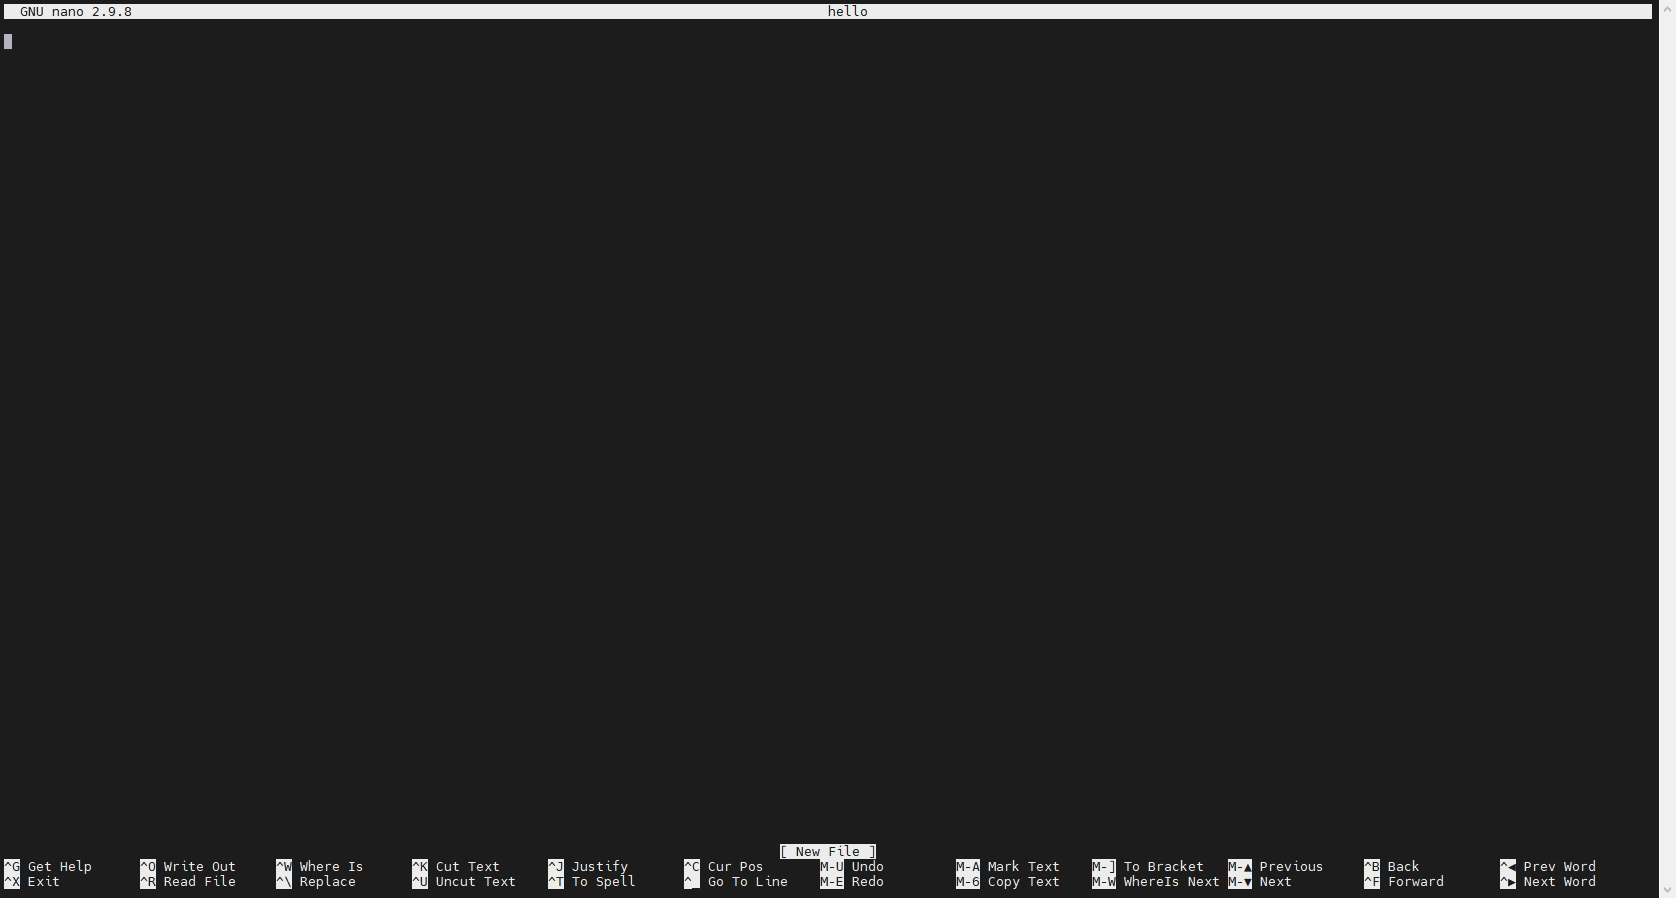
\includegraphics[width=1\linewidth]{Linux基础/文本编辑工具vi和vim/使用nano简单创建文件/fig/nano界面.png}
    \caption{nano界面}
    \label{fig:使用nano简单创建文件-nano界面}
\end{figure}

当打开时,软件默认就是\emph{编辑模式},你可以在里面随意输入一些内容,例如,输入“hello world”,屏幕上就是直接显示你的内容。对于删除和换行,其操作就如图在Windows下的记事本一样(使用键盘上下左右、删除键等)。重点是下面的菜单选项。难度本身也不大,只需要记住两个符号所表示的含义即可:\^表示键盘上的\code{Ctrl}键,而\code{M-}表示键盘上的\code{Alt}键。因此,正如你所看到的那样,在nano当中,使用\keywordin{nano}{Ctrl+X}退出;使用\keywordin{nano}{Ctrl+O}保存。

\begin{attention}
    在\code{nano}当中,一个很特殊的地方在于它的复制、剪切和粘贴与我们所熟悉的快捷键不一样。根据下面的说明,可以看到,复制是\keywordin{nano}{Alt+6},剪切是\keywordin{nano}{Ctrl+K},而粘贴是\keywordin{nano}{Ctrl+U}。

    同时,无论是复制还是剪切,默认都是\emph{对行进行操作}。也可以使用\keywordin{nano}{Alt+A}\footnote{这个命令可能和部分软件(如微信)的截图快捷键冲突。},并用方向键选中文本,进行操作。
\end{attention}

此外,\code{nano}也支持撤销(\keywordin{nano}{Alt+U})和恢复(\keywordin{nano}{Alt+E})。

\subsection{使用\code{nano}进行查找和替换}

几乎所有的文本编辑器,都需要有一些如\emph{查找}和\emph{替换}的功能方便我们进行编辑。在\code{nano}当中,查找的命令是\keywordin{nano}{Ctrl+W},此时下方会弹出一个输入框,输入要查找的内容,回车后光标便会定位在光标下方第一个匹配的开头位置。使用\keywordin{nano}{Alt+↓}和\keywordin{nano}{Alt+↑}可以切换到下一个匹配位置或上一个匹配位置。

\begin{attention}
    \code{nano}在匹配查找时不区分大小写,例如,想查找\code{SIGMA}时,在输入查找内容时输入\code{sigma}同样可以。
\end{attention}

对于替换功能,其命令为\keywordin{nano}{Ctrl+$\backslash$},此时首先弹出对话框,输入要查找的内容的,之后弹出的对话框输入要替换的内容。之后光标会从当前位置开始向后搜索,当查找到一个后会定位到此处并询问是否替换。输入\code{y}表示确认,输入\code{n}表示不替换此处。如果确认要全部替换的话,可以直接输入\code{a};相对地,如果发现有错(例如要查找的词语或要替换的词语拼写错了),可以输入\code{c}取消替换命令。

除此之外,还有更多的命令(例如查看字数是\keywordin{nano}{Alt+D}),可以直接使用\keywordin{nano}{Ctrl+G}查看帮助文档。在帮助文档中还包含有一些命令的快捷方式,例如查看文档除了可以使用\code{Ctrl+G}外,也可以直接使用\code{F1}键。

\begin{attention}
    \code{nano}的使用方法看似讲了很多,实际上只需要记住:\^表示键盘上的\code{Ctrl}键,而\code{M-}表示键盘上的\code{Alt}键,其他的,都可以通过下方的说明,或者帮助文档找到。
\end{attention}

\subsection{错误处理}\label{subsec:使用nano简单创建文件-错误处理}

\subsubsection{[ File <文件名> is unwritable ]}

这是因为你没有这个文件的可编辑权限。借助于\ref{subsec:文件权限管理-修改文件权限}一节所介绍的\code{chmod}命令可以添加可编辑权限。

\begin{attention}
    大多数时候,之所以这个文件不可编辑,是因为这个文件含有重要内容(可能是你误打了一个系统文件的路径,虽说这个可能性很小)。因此,遵守这个权限,不要修改是最好的。如果确实需要修改,仔细检查。
\end{attention}

\subsubsection{[ Error reading <文件名>: Permission denied ]}

这是因为你没有这个文件的可读权限,解决方法与上一个错误一样(使用\code{chmod}命令)

与前面的注意内容一样,遵守这个权限往往是最正确的选择。
% 请在下方的大括号相应位置填写正确的节标题和标签,以及作者姓名
\section{使用\keyword{vi},\keyword{vim}创建文件}\label{sec:使用vi,vim创建文件}
\sectionAuthor{Jiaqi Z.}

% 请在下方的item内填写本节知识点
\begin{Abstract}
    \item 如何通过\code{vi},\code{vim}创建并保存文件
    \item 如何通过\code{vi},\code{vim}打开已有文件
\end{Abstract}

% 请在正文相应位置填写正确的小节标题(或小小节标题),同时将标签的“节标题”和“小节标题”改为实际内容

\subsection{通过\code{vi}创建文件}\label{subsec:使用vi,vim创建文件-通过vi创建文件}

从本节开始,这一章就要开始讨论\code{vi}和\code{vim}的操作方法。类似于使用\code{nano}编辑文件,在Linux当中通过\code{vi}(\code{vim})创建文件的方法是\code{vi <文件名>}或\code{vim <文件名>}。通常来说,使用\code{vi}创建文件后的界面如图\ref{fig:使用vi,vim创建文件-vim界面}所示。

\begin{figure}
    \centering
    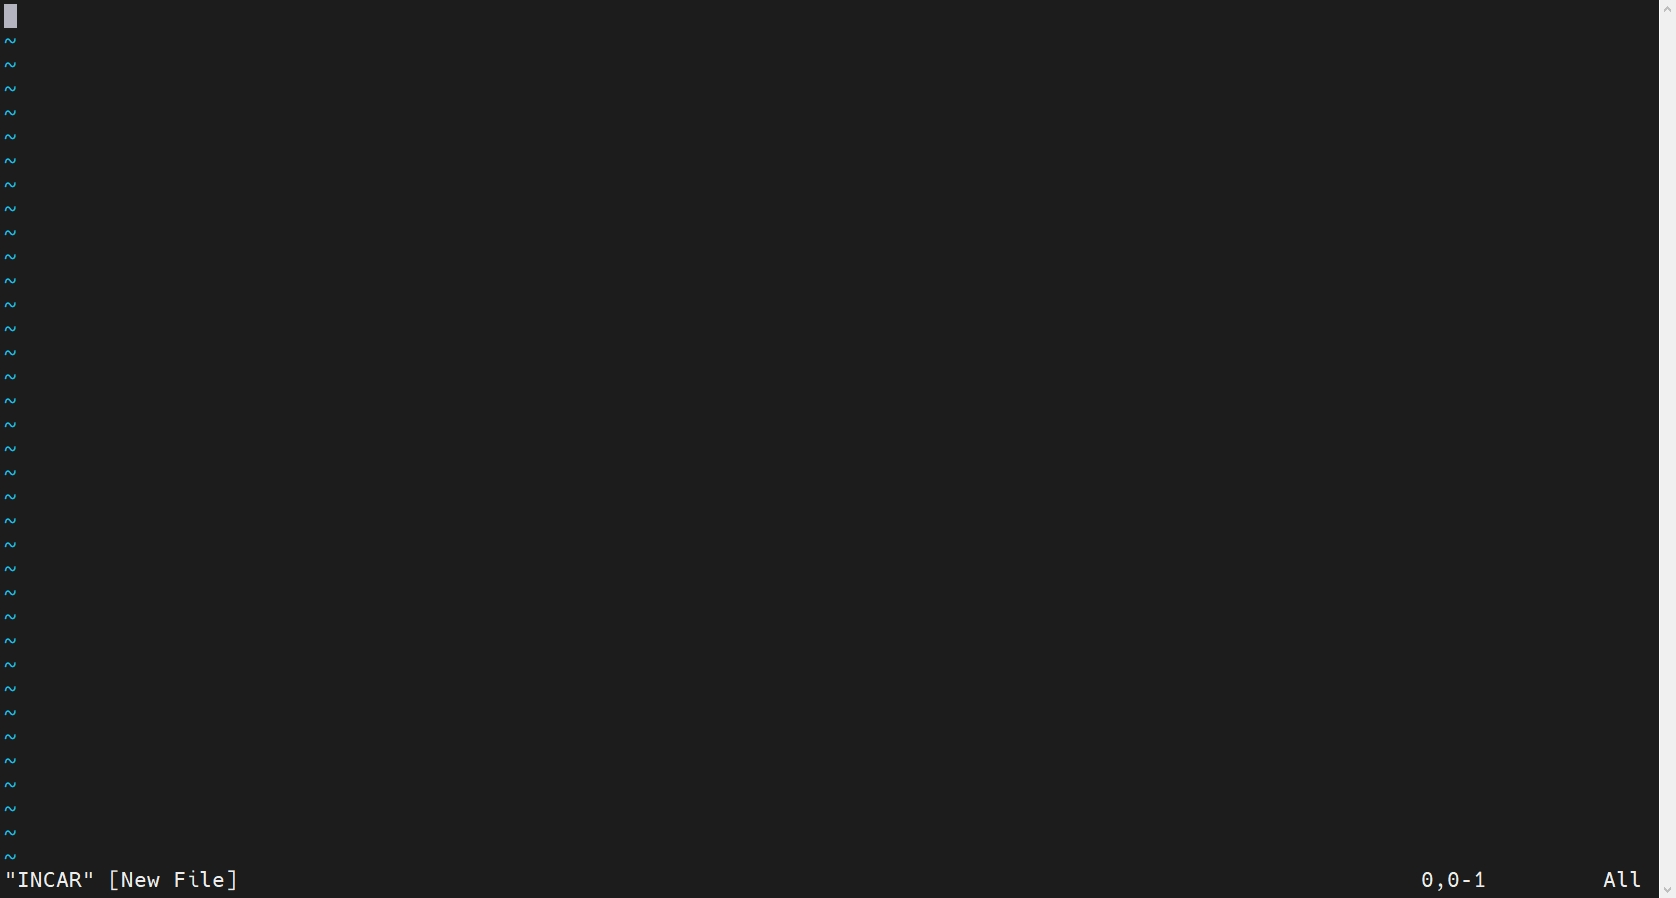
\includegraphics[width=1\linewidth]{Linux基础/文本编辑工具vi和vim/使用vi,vim创建文件/fig/vim界面.png}
    \caption{vim界面}
    \label{fig:使用vi,vim创建文件-vim界面}
\end{figure}

\begin{attention}
    仔细看图\ref{fig:使用vi,vim创建文件-vim界面}标题的话,可能会发现,明明说的是\code{vi}的创建文件,为什么显示的界面是\code{vim}呢?正如\ref{sec:使用nano简单创建文件}开头所说的那样,相比于vi,vim的功能更加强大。目前在很多操作系统当中,都是使用\code{vim}代替\code{vi}。因此,在本节标题中,我们使用\code{vi}和\code{vim}作为区分,在后面的讨论中,可能为了方便,我们使用\code{vi}代替\code{vim}(二者操作方法基本一致)。

    如果你确实想知道使用\code{vi}命令打开的是vim编辑器还是vi编辑器,可以使用\keyword{alias}命令,在输出中如果看到有\code{alias vi='vim'},那么说明实际上你所打开的是vim编辑器;如果没有,则意味着打开的是vi。此时如果希望打开vim编辑器,则需要使用命令\code{vim}代替\code{vi}。
\end{attention}

\subsection{vi编辑器的三种模式}\label{subsec:使用vi,vim创建文件-vi编辑器的三种模式}

与nano界面相比,vi界面显得更加“简洁”(没有了下方的菜单栏)。但是,如果你尝试着往里面输入内容的话,会发现往往不会是你想要的结果(也有可能“误打误撞”可以输入进去)。这是因为,在vi当中存在三种工作模式:

\subsubsection{普通模式}

当你使用\code{vi}命令打开编辑器后,则进入了编辑器的\emph{普通模式}。在这一模式下,你可以使用方向键移动光标,也可以进行删除、剪切、粘贴等简单操作。

一些简单的操作是使用\keywordin{vi}{x}键删除当前光标所在字符,使用\keywordin{vi}{dd}删除当前行(实际上是“剪切”),\keywordin{vi}{yy}复制当前行;使用\keywordin{vi}{p}(小写)将剪贴板内容粘贴到光标下方,\keywordin{vi}{P}大写表示粘贴到光标上方。\keywordin{vi}{u}表示撤销,\code{Ctrl+r}表示恢复撤销。

上面这些操作都是比较基础简单的,通常是用于对文件进行\emph{修改}的。而对于新创建的文件,则可以使用\keywordin{vi}{i}进入到“编辑模式”。同时,使用\keywordin{vi}{a}可以在光标下一个位置开始“编辑模式”,\keywordin{vi}{o}(小写字母)和\keywordin{vi}{O}(大写字母)分别表示在当前行下方和上方插入新的一行,并进入“编辑模式”

\subsubsection{编辑模式}

这是最熟悉的模式。可以在这一模式下如同正常文本编辑器一般进行编辑(例如,方向键移动光标,编辑字符,删除键等都是可用的)。除此之外,还有一些快捷键需要介绍一下\footnote{这些快捷键很多在Windows当中也有,但可能大多数人并不熟悉。}。

使用键盘上的\code{Home}键和\code{End}键可以将光标定位到行首和行尾;使用\code{Page Up}和\code{Page Down}可以上下翻页;使用\code{Insert}可以在“插入模式”和“替换模式”下切换。

在“编辑模式”下使用键盘上的\code{Esc}键可以返回到“普通模式”。

\subsubsection{命令行模式}

这一模式将会是最复杂的,许多vi的高级操作都是基于一系列的命令完成的。进入命令行模式的方法是\emph{在“普通模式”下输入键盘上的\code{:}}。

虽然大多数命令要在后面的章节提到它们,但一些必要的命令还是需要现在知道的--它们涉及到\emph{文件的保存}和\emph{编辑器的关闭}。例如,\keywordin{vi}{:w}表示保存文件,\keywordin{vi}{:q}表示关闭编辑器,\keywordin{vi}{:q!}表示强制退出(不保存),而\keywordin{vi}{:wq}表示保存后退出\footnote{它还有一个形式:\keywordin{vi}{:x}。}。

\subsection{通过\code{vi}打开已有文件}\label{subsec:使用vi,vim创建文件-通过vi打开已有文件}

类似于使用\code{nano <文件路径>}的方法,使用\code{vi}打开已有文件的方法是\code{vi <文件路径>}。与前面所介绍的内容一样,打开后的vi界面默认是“普通模式”,此时可以使用一些简单的方式(如\code{dd}删除整行等)对文件进行简单的编辑,或者可以使用“编辑模式”进行修改操作。

\begin{attention}
    在修改文件时,请确保是否有修改文件的权限。对于没有权限的文件进行修改,在退出时将会返回“'readonly' option is set (add ! to override)”的错误。

    正如错误中所说的那样,你可以使用\code{w!}的方式强行覆盖文件,但这始终是一种“下策”。
\end{attention}


\subsection{错误处理}\label{subsec:节标题-错误处理}
% 请在本节列出可能遇见的错误与解决方法

\subsubsection{E37: No write since last change (add ! to override) }

这表明你在\code{:q}退出时文件发生了修改。类似于WIndows操作系统下退出时询问是否保存一样,你需要选择是否保存你的编辑。如果保存,则需要先执行\code{:w}再\code{:q},或者直接执行\code{:wq};相对地,如果你不需要保存,则执行\code{:q!}强制退出。

\subsubsection{W10: Warning: Changing a readonly file}

这是一个警告信息,说明你正在编辑一个对你而言有权限限制的文件(大多数时候是“只读”文件,但对于某些“不可读”文件,如果强行编辑,可能也会引起该错误)。如果无视编辑并保存的话,通常会引发下面的错误:

\subsubsection{E45: 'readonly' option is set (add ! to override) }

这是正文最后所提到的错误,说明你编辑了一个有权限限制的文件。使用\code{:w!}可以强行覆盖保存文件,但这并不是一个正确的方法(至少是不推荐的方法)。

\subsubsection{ [Permission Denied] }

这是因为你在查看一个不可读的文件。当你尝试编辑时,则会引发上面的警告或错误。
\section{查找与替换}\label{sec:查找与替换}
\sectionAuthor{Jiaqi Z.}

\begin{Abstract}
    \item 使用\code{vi}的\code{/}和\code{?}进行字符串查找
    \item 使用\code{vi}进行字符串的替换
\end{Abstract}

对于一个现代文本编辑器,一个最基本的功能就是对某一特定的字符串进行查找,以及将其替换为另一字符串。相比于其他在Windows操作系统中常见的文本编辑器(无论是记事本、word、还是VS Code等),Linux的vi编辑器下的查找和替换都显得更加复杂。这确实可能带来了一些学习上的困难,但随着使用场景逐渐复杂,你会发现这种代码式的操作的便利性。

\subsection{查找}\label{subsec:查找与替换-查找}

首先先来了解如何对一个字符串进行查找。在vi当中,查找的方法是使用\keywordin{vi}{/}或者\keywordin{vi}{?},其基本格式为\code{/[要查找的字符串]}或者\code{?[要查找的字符串]}。例如,在当前文件中查找\code{Hello},可以输入\code{/Hello},然后回车。

\begin{attention}
    在输入字符串时,vi会同时在文本内将所有匹配的字符串进行高亮(即便没有按回车)。

    \code{/}和\code{?}的作用都是查找字符串,二者的区别在于,\code{/}是从当前光标开始向后查找,而\code{?}是向前查找。当输入完成后,点击回车,光标会自动定位到最近的相应位置。若要切换,则可以使用\keywordin{vi}{n}查找下一个或者使用\keywordin{vi}{N}查找上一个。
\end{attention}

\subsection{替换}\label{subsec:查找与替换-替换}

相比于查找命令,vi中的替换命令就显得更加复杂了。最基本的命令是\keywordin{vi}{s},但通常会配以更多的命令(类似于参数)。一般来说,替换命令可以用下面的方式表示:\code{:<开始行号>,<结束行号>s[分隔符][要替换的字符串][分隔符][替换为的字符串][分隔符]<g>}。其中\code{<开始行号>}和\code{<结束行号>}都是可选的,若省略则表示\emph{只对当前行进行替换}。命令结尾的\code{<g>}也是可选的,表示对所有进行替换,若省略则只替换第一个(每一行或当前行,取决于是否有行号)。

同时,在替换时需要使用\code{[分隔符]}对字符串进行分割,通常情况下习惯于使用\code{/}表示,但在一些特殊的情况下(例如要替换的字符串内带有这一字符),则可能会将其改为其他分隔符。命令当中所有出现分隔符的地方都需要\emph{统一}。

下面是一些例子,例如,若希望将当前行的\emph{第一个}“hello”替换为“bye”,则需要命令\code{:s/hello/bye/},若希望对所有字符串进行替换,则使用\code{:s/hello/bye/g}。

若希望对第一行到第三行的所有“hello”进行替换,则使用\code{:1,3s/hello/bye/g},若没有最后的\code{g},则表示仅对\emph{第一行到第三行每一行里面的第一个字符串进行替换}。

如果希望对第一行到最后一行的所有“hello”进行替换,则使用\code{:1,\$s/hello/bye/g}。其中,\keywordin{vi}{\$}表示\emph{最后一行}。

\begin{attention}
    在vi当中,数字可以具有\emph{重复若干次}的含义。例如,在前面所介绍的\code{x}表示删除当前光标所在字符,若前面加上一个数字,则表示重复这一操作多少次(即删除多少字符),例如,\code{10x}表示删除10个字符。

    同时,在vi当中,往往使用\code{\$}表示\emph{最后}的意思。例如,在普通模式下直接输入\code{\$}则直接跳转到\emph{这一行最后一个字符},类似的,输入\code{0}则跳转到这一行第一个字符。输入\code{:\$}可以直接跳转到文件最后一行。
\end{attention}


\subsection{错误处理}\label{subsec:查找与替换-错误处理}
% 请在本节列出可能遇见的错误与解决方法

\subsubsection{查找(替换)完之后字符串总是高亮显示,怎么将其关闭}

使用\code{:noh}命令。

\subsubsection{E488: Trailing characters}

这可能是在输入命令时使用了错误的格式。请仔细检查使用的命令(尤其是替换命令)的格式

\subsubsection{想要替换,却发现把光标上的字符删除了}

这是因为在使用替换命令时,前面需要有冒号\code{:}。若没有添加这一符号,直接使用\keywordin{vi}{s}则意味着\emph{删除当前字符并插入}
\section{初窥正则表达式}\label{sec:初窥正则表达式}
\sectionAuthor{Jiaqi Z.}

\begin{Abstract}
    \item 什么是正则表达式
    \item 如何使用简单的正则表达式进行查找和替换
\end{Abstract}

\subsection{关于正则表达式}\label{subsec:初窥正则表达式-关于正则表达式}

在\ref{sec:查找与替换}一节当中,我们提到过,vi的查找和替换相比于其他文本编辑器都稍显复杂。而这一节所介绍的\emph{正则表达式},则是其十分强大的功能之一。

简单来说,正则表达式是\emph{一种用于匹配和操作文本的强大工具,它是由一系列字符和特殊字符组成的模式,用于描述要匹配的文本模式}。借助于正则表达式,我们可以很方便对许多具有相同模式的字符串进行匹配与处理。例如,对于\code{ENCUT=200}和\code{ENCUT=400},从字符串本身来看是不同的,但二者具有相同的模式(\code{ENCUT=}加上一系列整数字符)。因此,可以使用正则表达式进行批量处理。

在Linux当中,正则表达式是相对比较复杂的内容。在这一节只是简单介绍一下基本用法,对于更完整的内容,将在后面章节进行介绍。

\subsection{元字符}\label{subsec:正则表达式-元字符}

正则表达式最有特色的部分,就是可以使用\emph{元字符}来匹配一系列特定的字符。在介绍一些复杂的元字符之前,先熟悉一个最简单的符号,\code{[]},在中括号里面,可以放入一些字符。正则表达式将会\emph{匹配这些字符当中的一个}。例如,对于字符串“hello”,使用正则表达式\code{[aeiou]}就可以匹配到字符串里面的所有元音字母。

\begin{attention}
    在vi当中,可以使用正常的查找方式和替换方式,只不过需要在输入查找的内容时使用正则表达式。简单说,你可以将正则表达式看作是一个表达多个字符串集合的方式,而可以使用这种方式一次性对这个集合内的每一个元素进行查找和替换。这样的话,其使用方法就与普通的查找和替换基本无异了。

    同时,特别需要注意的一点是,在vi当中,有一些符号(后面会提到)与Linux本身的正则表达式不同(Linux的命令行本身也是支持正则表达式的),通常区别在于是否添加一个反斜杠(\code{$\backslash$})。后面遇到时会特别指出。
\end{attention}

在上面的例子中,我们可以直接在vi当中直接使用\code{/[aeiou]}实现对所有元音字母的查找。

在使用\code{[]}时,可以使用\code{-}对特定范围内的字符进行查找。例如,使用\code{[a-h]}表示对a到h之间的所有字母(小写字母)进行查找。常用的还有,使用\code{[A-Z]}表示对所有大写字母进行匹配,\code{[a-z]}表示对小写字母进行匹配,\code{[0-9]}表示对所有阿拉伯数字进行匹配。

\begin{extend}
    也许你会有疑问:这个范围是按照什么排序的?在计算机当中,这些字符都是根据ASCII码将其转化为二进制存储在计算机内。因此,这里的排序也是根据每一个字符所对应的ASCII码排序的。

    ASCII(American Standard Code for Information Interchange,美国信息交换标准代码)是基于拉丁字母的一套电脑编码系统。它主要用于显示现代英语,而其扩展版本延伸美国标准信息交换码则可以部分支持其他西欧语言,并等同于国际标准ISO/IEC 646。

    ASCII 由电报码发展而来。第一版标准发布于1963年 ,1967年经历了一次主要修订,最后一次更新则是在1986年,至今为止共定义了128个字符;其中33个字符无法显示(一些终端提供了扩展,使得这些字符可显示为诸如笑脸、扑克牌花式等8-bit符号),且这33个字符多数都已是陈废的控制字符。控制字符的用途主要是用来操控已经处理过的文字。在33个字符之外的是95个可显示的字符。

    例如,0的ASCII码为48,A的ASCII码为65,而a的ASCII码为97。因此,可以使用\code{[0-a]}匹配到大写字母\code{A}。
\end{extend}

同时,中括号里面的字符是可以组合使用的,例如,可以使用\code{[A-Za-z]}表示所有的字母。那如果希望表达所有的字母和数字呢?

\answer{\code{[A-Za-z0-9]}}

除此之外,对于一些常见的字符,为其设置了特殊的符号,例如,\code{$\backslash$d}就表示\emph{所有的数字字符},\code{$\backslash$w}表示\emph{所有的字母、数字和下划线},也就等价于\code{[A-Za-z0-9\_]}。

而在使用中括号时,也可以使用符号\code{\^}进行\emph{反选}。例如,使用\code{\^[A-Z]}表示排除所有大写字母的字符。

\subsection{总结}\label{subsec:初窥正则表达式-总结}

本节简单介绍了一些常见的元字符,并可以将其用于查找和替换。例如,在本节开头所介绍的\code{ENCUT=200}和\code{ENCUT=400},使用正则表达式可以直接表示为:\code{ENCUT=$\backslash$d$\backslash$d$\backslash$d}\footnote{事实上,它还有更简洁的表示方法\code{ENCUT=$\backslash$d$\backslash$+},但碍于本节的内容,详细的含义将放在后面章节介绍。}。

正如最开始所说的那样,正则表达式的功能远不止此,对于更复杂的部分(例如,目前使用\code{[]}只能匹配一个字符,如何匹配多个字符?),将在后面的章节进行更加详细的介绍。

\subsection{错误处理}\label{subsec:初窥正则表达式-错误处理}

\subsubsection{如何查找如\code{[hello]}这样的字符串?}

在正则表达式当中,已经将中括号作为特殊符号使用。因此,如果想查找带有中括号的字符串,则需要将中括号前面添加一个反斜杠\code{$\backslash$}表示中括号这一字符本身。例如,对于上面的例子,如果直接使用\code{[hello]}表示匹配这5个字母(实际为4个)当中的任意一个字符;而使用\code{$\backslash$[hello$\backslash$]}或者\code{$\backslash$[hello]}都可以表示字符串“[hello]”

    \part{VASP计算}

    \chapter*{写在前面的一些说明}

从本部分开始,就进入到了这一教程的主体部分--\emph{VASP计算}。在开始计算之前,有一些注意事项需要说明:

\section*{关于输入文件}

随着计算任务的不同,VASP所需要的输入文件也是不同的。对于\code{INCAR}和\code{KPOINTS}文件\footnote{这些文件的具体含义在后续教程中都会详细介绍。},通常是与具体的计算任务有关,且可以借助于如vaspkit的脚本生成。而对于\code{POSCAR}文件而言,其表示所要计算的结构信息,对于不同的课题组、不同的研究课题,所研究的结构也会千差万别。在教程中为了演示方便,有时会设定某一特定的结构作为\code{POSCAR}文件,仅作为演示用,在实际使用时需要根据具体问题设置不同的文件。

对于\code{POTCAR}文件而言,通常对于已经购买版权的课题组而言,都会有一个配套的\code{POTCAR}目录,里面会包含有所有元素的赝势文件。对于这种情况,通常使用如vaspkit的脚本生成并不是难事(同样也可以使用Linux命令手动生成,具体内容在后续章节会进行介绍)。对于没有购买版权的课题组来说,可以“暂时借用”别人已有的文件\emph{作为练习},但不能将其用于课题组的论文当中。

\section*{关于提交脚本}

之前所介绍的Linux命令,在大多数课题组的系统中都是可以使用的。但VASP却不是如此。首先,不同课题组的VASP版本可能不同,有时不同版本的命令或参数含义可能会有些许变化,但这种变化通常是影响较小的。最重要的是,由于所使用的系统环境不同,例如,对于本地运行和运算集群运行,其提交任务的方法可能会有些许差异。目前,大多数课题组在计算VASP任务时都是采用服务器集群进行计算,此时就会需要一个叫做\emph{排队系统}的东西。

对于不同课题组的不同集群,所使用的排队系统可能不同。本教程在编写时,通常是使用slurm作业管理系统,目前如中国科学技术大学、上海交通大学等学校的计算中心都是采用这一管理系统。对于使用其他管理系统的课题组而言,需要参考自己课题组的使用方法。

\section*{使用slurm的命令与方法}

考虑到教程的完整性,这一节简单介绍关于slurm的命令。

\begin{attention}
    这一部分仅仅适用于那些使用slurm作业管理系统的课题组,对于其他课题组,则需要参考自己课题组的使用方法。
\end{attention}

在使用slurm时,需要配合以一个提交任务脚本。一个典型的提交任务脚本\code{sub.vasp}如下所示:

\begin{lstlisting}[caption=sub.vasp]
#!/bin/bash
#SBATCH -n 56
#SBATCH -N 1

# 打印任务信息
echo "Starting job $SLURM_JOB_ID at " `date`
echo "SLURM_SUBMIT_DIR is $SLURM_SUBMIT_DIR"
echo "Running on nodes: $SLURM_NODELIST"

# 执行任务
## 载入vasp
module load VASP
ulimit -s unlimited
mpirun vasp_std > vasp.out 2>vasp.err

# 任务结束
echo "Job $SLURM_JOB_ID done at " `date`
\end{lstlisting}

其中,\code{\#SBATCH -n}表示\emph{任务所使用的核数},在本例中设定为56核;\code{\#SBATCH -N}表示\emph{使用的节点数}。在上述代码中,表示使用56核,1个节点进行计算。

而对于中间的命令,特别的如\code{ulimit -s unlimited}表示\emph{不设置内存限制};\code{mpirun vasp\_std > vasp.out 2>vasp.err}表示通过\code{mpirun}(即\emph{并行计算程序})运行\code{vasp\_std}命令并将输出结果保存至\code{vasp.out},而将错误信息输出到\code{vasp.err}当中。

\begin{extend}
    对于有显卡加速的课题组而言,可能需要在前面指定\code{\#SBATCH --partition=GPU}指定使用的GPU(如\code{a100}等),同时使用\code{\#SBATCH --gres=gpu:$n$}表示调用$n$张显卡进行计算。
\end{extend}

提交任务时,需要将提交脚本和计算目录放在一起,在计算目录下使用\keyword{sbatch}\code{ sub.vasp}\footnote{提交脚本名}即可。除此之外,slurm还有如下命令:

\begin{itemize}
    \item \keyword{squeue}表示查看当前任务队列
    \item \keyword{scancel [jobID]}表示取消\code{[jobID]}编号的任务,例如,\code{scancel 6066}表示取消编号为6066的任务;
\end{itemize}

除此之外,slurm也可以使用如\code{srun}或\code{salloc}提交交互式作业,或者申请特定的资源并登录至节点。这一部分内容在VASP计算时不会使用到,因此不在这里介绍。
% \chapter{写在前面}\label{chap:写在前面}
\minitoc
\section{宇宙级免责声明}\label{sec:宇宙级免责声明}

是的,这一小节本来应该称作 前言 的,但是我怕你跳过不看所以特地用了有趣的名字。

本节的内容虽然不正式但是非常严肃,是笔者作为一个小白吃了N堑之后所得的心血感言,也是为读者更好地使用本书轻轻推开计算领域的大门所做的铺垫,更是为后续进入材料计算领域的朋友们预留的忠告。

官网

论坛

本书涉及领域较少

软件仅介绍使用到的功能
111
% \chapter{电子性质}\label{chap:电子性质}
\minitoc
\section{能带}\label{sec:能带}
\chapter{能带计算}\label{chap:能带计算}
\minitoc
% 请在下方的大括号相应位置填写正确的节标题和标签,以及作者姓名
\section{能带基础理论}\label{sec:能带基础理论}
\sectionAuthor{Jiaqi Z.}

% 请在下方的item内填写本节知识点
\begin{Abstract}
    \item 什么是能带
    \item 能带的三个重要近似
\end{Abstract}

在本章,我们将要了解材料计算的一个重要内容--关于能带的计算。毫不夸张地说,能带论是目前研究固体中的电子状态,说明固体性质最重要的理论基础。一个最简单的例子是,利用能带的相关计算,我们可以从严格的角度判断材料的导电性。

\begin{extend}
    导体和绝缘体的概念,贯穿了我们的学习生涯。而这一概念也在随着认知水平的增长发生变化。

    最开始接触的时候,我们认为,导体是那些带有电荷的物质,而绝缘体内部没有电荷。这一结论是我们对“电”和“电荷”的初步认识,显然是不准确的。进一步学习了物理后,我们了解到:任何原子都是由原子核和电子组成的,所谓的导体,就是存在“自由移动的电子”,相反,绝缘体就是没有自由电子的物质。这一概念结合了原子和电子的认识,相比于最开始的“电荷”,显然更准确了。

    到了现在,我们将要了解到能带。基于能带理论,在导体中,价带(价电子所在的能带)和导带(电子可以自由移动的能带)是重叠的,或者价带顶部和导带底部之间的能隙(带隙)非常小,甚至为零。这意味着电子可以轻易地从价带跃迁到导带,从而在电场作用下自由移动,形成电流。而对于半导体而言,价带和导带之间存在一个较大的带隙,电子要跃迁到导带需要吸收足够的能量(如热能或光能)。在常温下,电子通常没有足够的能量来跃迁,因此电子不能自由移动,导致绝缘体不导电。
\end{extend}

\subsection{什么是能带}\label{subsec:能带理论基础-什么是能带}

从原子物理的知识来看,一个孤立原子的电子只能处在特定的能级当中。而我们所计算的材料,往往是周期性的多原子材料\footnote{对于VASP而言,所有材料都是“周期性”的。我们所说的单原子或单分子计算,通常是通过调整晶格的大小,从而减弱相互之间的作用,近似成“单分子”计算。}。对于多原子而言,电子和电子之间、电子和原子核之间会产生相互作用,此时电子的能级就会发生“展宽”,从而变成一系列的带状结构。称为“能带”。

\begin{attention}
    通常情况下,能带仅在周期性材料中讨论。对于单分子(如气体分子等),计算能带往往没有意义。
\end{attention}

% \subsubsection{小小节标题}

\subsection{能带理论的三个近似}\label{subsec:能带理论基础-能带理论的三个近似}

我们不会在这一教程中详细介绍能带的推导过程,但是我们还是有必要在这里提到三个重要的近似。这些近似可以说是能带理论的基础,甚至可以说是整个第一性原理计算的基础。

\begin{itemize}
    \item Born-Oppenheimer近似,又名绝热近似:因为原子核比电子重的多,所以原子核比电子具有更大的惯性,更难运动。因此,我们只考虑电子的运动,原子核是被固定住的。
    \item 单电子近似(独立电子近似、平均场近似):将电子与电子相互作用等效成一个平均值,电子是在一个平均场中运动。
    \item 周期场近似:平均场是周期性的。
\end{itemize}

具体内容在任何一本固体物理教材中都会详细提到,这里不再赘述。
% 请在下方的大括号相应位置填写正确的节标题和标签,以及作者姓名
\section{VASP计算能带过程}\label{sec:VASP计算能带过程}
\sectionAuthor{Jiaqi Z.}

% 请在下方的item内填写本节知识点
\begin{Abstract}
    \item 如何使用VASP计算PBE能带
\end{Abstract}

在本节,我们将详细讨论如何使用VASP计算能带。我们先讨论最简单的PBE能带计算过程,旨在通过这一流程,掌握计算能带的完整步骤。在这一基础上,后面将会详细讨论精度更高的计算方法(如HSE能带计算等)。

\begin{attention}
    使用PBE计算能带往往会得到较小的带隙,如果你使用数据库或文献中的能带图进行复现,可能会得到与文献不同的带隙。这一点是PBE泛函计算能带所固有的缺陷,
\end{attention}

\subsection{结构优化}\label{subsec:VASP计算能带过程-结构优化}

在这一部分计算能带时我们使用\ch{SiO2}为例进行分析。所使用数据库来源自Materials Project\footnote{https://legacy.materialsproject.org/materials/mp-546794/}。

\ch{SiO2}的结构文件\code{POSCAR}如下所示:

\begin{lstlisting}[caption=POSCAR]
Si2 O4
1.0
        5.1358423233         0.0000000000         0.0000000000
        0.1578526541         5.1334159104         0.0000000000
        -2.6468476750        -2.5667081359         3.5753437737
    Si    O
    2    4
Direct
        0.750000000         0.250000000         0.500000000
        0.000000000         0.000000000         0.000000000
        0.787033975         0.625000000         0.662033975
        0.875000000         0.212965995         0.837966025
        0.962966025         0.125000000         0.337965995
        0.375000000         0.037034001         0.162034005
\end{lstlisting}

\begin{attention}
    在计算能带时,大多数时候我们只讨论原胞的计算。因此,在使用Materials Project等数据库导出结构时,应当优先导出原胞结构(Primitive Cell)。

    对于无法导出原胞的情况,可以借助于其他程序或脚本文件。以vaspkit为例,借助于\code{vaspkit-602},可以得到\code{PRIMCELL.vasp}文件,将其重命名为\code{POSCAR}文件即可。
\end{attention}

\begin{extend}
    对于一些特殊情形(例如需要掺杂等情况),不得不使用超胞进行计算。如果确实需要计算能带结构,往往需要对能带进行\emph{反折叠}以得到更清楚的图像。我们将在后面的部分对这一技术进行讨论。

    目前,我们所讨论的结构都是原胞。
\end{extend}

在计算能带之前,首先需要对材料进行结构优化。为得到结构优化所用\code{INCAR}文件,使用\code{vaspkit-101-LR}生成。同时调整其中的部分参数,修改后的\code{INCAR}文件如下:

\begin{lstlisting}[caption=INCAR]
Global Parameters
ISTART =  1
LREAL  = .FALSE.
ENCUT  =  600
PREC   =  Accurate
LWAVE  = .TRUE.
LCHARG = .TRUE.
ADDGRID= .TRUE.
    
Lattice Relaxation
NSW    =  300
ISMEAR =  0
SIGMA  =  0.05
IBRION =  2
ISIF   =  3
EDIFFG = -1.5E-02
\end{lstlisting}

其中,需要特别注意并调整的是:

\begin{itemize}
    \item \keyword{ENCUT}:截断能。通常设置为600或更高,但更高的截断能往往意味着更长的机时。同时,在后续所有计算中,截断能应当保持不变。
    \item \keyword{ISIF}:表示优化方式。对于一般的结构优化,通常设置为\code{ISIF=3}表示\emph{优化原子坐标和晶格参数}。对于一些特殊的材料(如二维材料),一些晶格参数可能不希望发生变化,此时可以设置\keyword{OPTCELL}文件,其内容为$3\times3$的矩阵,分别对应\code{POSCAR}当中的晶格参数坐标。其元素可以是0(表示不优化该坐标)或1(表示优化该坐标)。对于晶格参数不变的情况,可以设置为\code{ISIF=2}表示\emph{只优化原子坐标}。
    \item \keyword{EDIFFG}:表示优化收敛标准。其中正数表示\emph{能量收敛标准}(即能量变化小于这一数值时停止计算),而负数表示\emph{力收敛标准}(原子作用力小于这一数值的绝对值时停止计算)。
    \item \keyword{NSW}:表示\emph{最大离子步}。当优化离子步达到设定数值时停止计算(此时往往未达到收敛标准,需要重新计算)。或者,当\code{EDIFFG=0}时,计算达到设定\code{NSW}时停止计算。
\end{itemize}

对于\code{KPOINTS}文件,在结构优化时可以使用“自洽计算”的K点,使用\code{vaspkit-102}生成,通常设定Gamma点(2),选择密度时通常设定为0.02-0.04即可。

本例使用\code{vaspkit-102-2-0.02}生成\code{KPOINTS}文件如下所示:

\begin{lstlisting}[caption=KPOINTS]
K-Spacing Value to Generate K-Mesh: 0.020
0
Gamma
  12  12  14
0.0  0.0  0.0
\end{lstlisting}

\begin{attention}
    使用vaspkit生成K点的同时,脚本会同步生成赝势文件\code{POTCAR}。但为了确保生成文件的正确性,建议使用\code{grep TITEL POTCAR}查看赝势文件是否正确(与\code{POSCAR}文件相比较)\footnote{我也不知道为什么它是“TITEL”而不是“TITLE”,如果实在记不住的话用\code{TIT}也能搜索到对应内容。}。
\end{attention}

将以上文件放置在一个目录下,提交任务计算后得到\code{CONTCAR}文件,即为优化后得到的结构文件。

\subsection{自洽计算}\label{subsec:VASP计算能带过程-自洽计算}

计算完成后,新建一个目录(例如命名为\code{scf}),将结构优化得到的\code{CONTCAR}文件复制(或移动)到\code{scf}目录内,并重命名为\code{POSCAR}。

将结构优化的\code{KPOINTS}和\code{POTCAR}复制(或移动)到\code{scf}目录内。

使用\code{vaspkit-101-ST}命令生成自洽计算所需要的\code{INCAR}文件。其中需要将截断能\code{ENCUT}设置为结构优化所使用的标准。修改后得到的\code{INCAR}文件如下所示:

\begin{lstlisting}[caption=INCAR]
Global Parameters
ISTART =  1
LREAL  = .FALSE.
ENCUT  =  600
PREC   =  Accurate
LWAVE  = .FALSE.
LCHARG = .TRUE. 
ADDGRID= .TRUE. 

Static Calculation
ISMEAR =  0
SIGMA  =  0.05
LORBIT =  11
NEDOS  =  2001
NELM   =  60
EDIFF  =  1E-08
\end{lstlisting}

其中需要特别注意的设置是:

\begin{itemize}
    \item \keyword{LWAVE}:表示写入波函数文件\code{WAVECAR},通常用于继续计算时的初始化设定。由于文件较大,因此如无必要,通常可以将其设定为\code{.FALSE.}表示不写入文件。
    \item \keyword{LCHARG}:表示写入电荷密度文件\code{CHGCAR}。在计算能带时,由于需要使用到这一文件,因此需要将其设定为\code{.TRUE.}。
    \item \keyword{EDIFF}:表示电子收敛标准。当能量变化达到这一标准时结束迭代计算。
\end{itemize}

将所有文件准备好后提交任务。

\subsection{能带计算}\label{subsec:VASP计算能带过程-能带计算}

相比于自洽计算,能带计算所需要的K点是特殊的\emph{高对称点路径},因此关键在于KPOINTS的生成。

将自洽计算得到的\code{CHGCAR}, \code{POSCAR}, \code{INCAR}, \code{POTCAR}全部复制(或移动)到一个新的目录下(假设为\code{band})。

使用\code{vaspkit-3}生成计算能带所用\code{KPOINTS}文件。其中需要根据结构特点选择是二维材料还是三维材料,在本例中由于\ch{SiO2}是二维材料,因此使用\code{KPOINTS-303}生成\code{KPATH.in}文件,将其命名为\code{KPOINTS}文件。生成后得到的文件如下所示。

\begin{lstlisting}[caption=KPOINTS]
K-Path Generated by VASPKIT.
   20
Line-Mode
Reciprocal
   0.0000000000   0.0000000000   0.0000000000     GAMMA          
   0.0000000000   0.0000000000   0.5000000000     X              
 
   0.0000000000   0.0000000000   0.5000000000     X              
   0.2500000000   0.2500000000   0.2500000000     P              
 
   0.2500000000   0.2500000000   0.2500000000     P              
   0.0000000000   0.5000000000   0.0000000000     N              
 
   0.0000000000   0.5000000000   0.0000000000     N              
   0.0000000000   0.0000000000   0.0000000000     GAMMA          
 
   0.0000000000   0.0000000000   0.0000000000     GAMMA          
   0.5000000000   0.5000000000  -0.5000000000     M              
 
   0.5000000000   0.5000000000  -0.5000000000     M              
   0.3674577537   0.6325422463  -0.3674577537     S              
 
  -0.3674577537   0.3674577537   0.3674577537     S_0            
   0.0000000000   0.0000000000   0.0000000000     GAMMA          
 
   0.0000000000   0.0000000000   0.5000000000     X              
  -0.2349155075   0.2349155075   0.5000000000     R              
 
   0.5000000000   0.5000000000  -0.2349155075     G              
   0.5000000000   0.5000000000  -0.5000000000     M              
\end{lstlisting}

其中每相邻两个点都是对应于一条高对称点路径。

对于\code{INCAR}文件,需要在自洽所使用文件的基础上,添加\code{ICHARG=11}表示\emph{读取当前目录下的\code{CHGCAR}文件},从而用于非自洽计算。

\begin{extend}
    在这里我们提到了\emph{自洽计算}和\emph{非自洽计算},简单来说,自洽计算就是用来计算电子结构最稳定状态,而非自洽计算则是利用这一结构计算电子的其他性质(如能带、态密度等)。
\end{extend}

将以上文件整理后提交任务计算。至此我们就已经完成了VASP计算能带的所有过程。


% \subsection{错误处理}\label{subsec:节标题-错误处理}
% % 请在本节列出可能遇见的错误与解决方法

% \subsubsection{错误1}

% \subsubsection{错误2}

% \subsubsection{错误3}
% 请在下方的大括号相应位置填写正确的节标题和标签,以及作者姓名
\section{能带绘图与后处理}\label{sec:能带绘图与后处理}
\sectionAuthor{Jiaqi Z.}

% 请在下方的item内填写本节知识点
\begin{Abstract}
    \item 如何使用Origin绘制能带图
    \item 如何使用vaspkit自动生成能带图
\end{Abstract}

% 请在正文相应位置填写正确的小节标题(或小小节标题),同时将标签的“节标题”和“小节标题”改为实际内容

在上一节的计算中,我们已经得到了能带所需要的全部信息。但是,使用计算软件得到的仅仅是数据,与我们所需要的“\emph{能带图}”还差一个步骤--数据后处理。

在这一节,我们将讨论如何借助于vaspkit软件绘制能带图。其中,最基本的方法是使用Origin绘图,但在vaspkit的更新过程中,也添加了借助于Python脚本自动绘图的功能。我们将在本节首先介绍如何配置可自动绘图的vaspkit,然后介绍如何使用vaspkit自动绘图。

\begin{attention}
    vaspkit自动绘图并不一定在所有版本都可用,同时这依赖于服务器的配置是否有必要的包(如Python,matplotlib等)。因此,你不应当将vaspkit自动绘图作为依赖,而是作为一个“备选项”。

    使用Origin绘图应当是绘制能带图首先需要掌握的内容。
\end{attention}

\subsection{使用Origin绘制能带图}\label{subsec:能带绘图与后处理-使用Origin绘制能带图}

使用Origin绘制能带图的第一步是\emph{得到能带图上每一点的坐标},借助于vaspkit我们可以很容易实现。利用\code{vaspkit-211}可以得到绘制能带图所需要的\code{BAND.dat}文件,其中包含了能带图的数据点坐标,下面则是文件开始的一部分:

\begin{lstlisting}[caption=BAND.dat]
#K-Path(1/A) Energy-Level(eV)
# NKPTS & NBANDS: 180  64
# Band-Index    1
    0.00000    -19.370800
    0.04630    -19.368108
    0.09260    -19.360010
    0.13890    -19.346551
    0.18520    -19.327775
    0.23150    -19.303736
    0.27780    -19.274533
\end{lstlisting}

除此之外,我们还会得到\code{KLINES.dat}文件,用于生成高对称点坐标。将这两个文件下载到本地后,导入Origin软件当中。在\code{BAND.dat}文件后新添一列,并将\code{KLINES.dat}文件复制到新添的列中,得到的文件如图\ref{fig:能带绘图与后处理-BAND.dat修改后}所示。

\begin{figure}
    \centering
    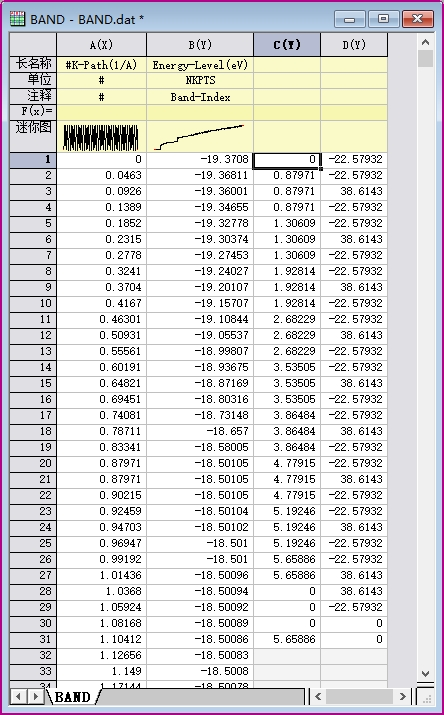
\includegraphics[width=1\linewidth]{VASP计算/能带计算/能带绘图与后处理/fig/BAND_dat.png}
    \caption{\code{BAND.dat}修改后}
    \label{fig:能带绘图与后处理-BAND.dat修改后}
\end{figure}

将新添加的C列(\code{KLINES.dat}文件中的x坐标的属性设置为“X”(方法:右键点击上方列名-“设置为”-X)

将这4列数据全选后点击菜单栏“绘图”-“基础2D图”-“折线图”即可得到所绘制的能带如图\ref{fig:能带绘图与后处理-Origin生成的能带图}所示。

\begin{figure}
    \centering
    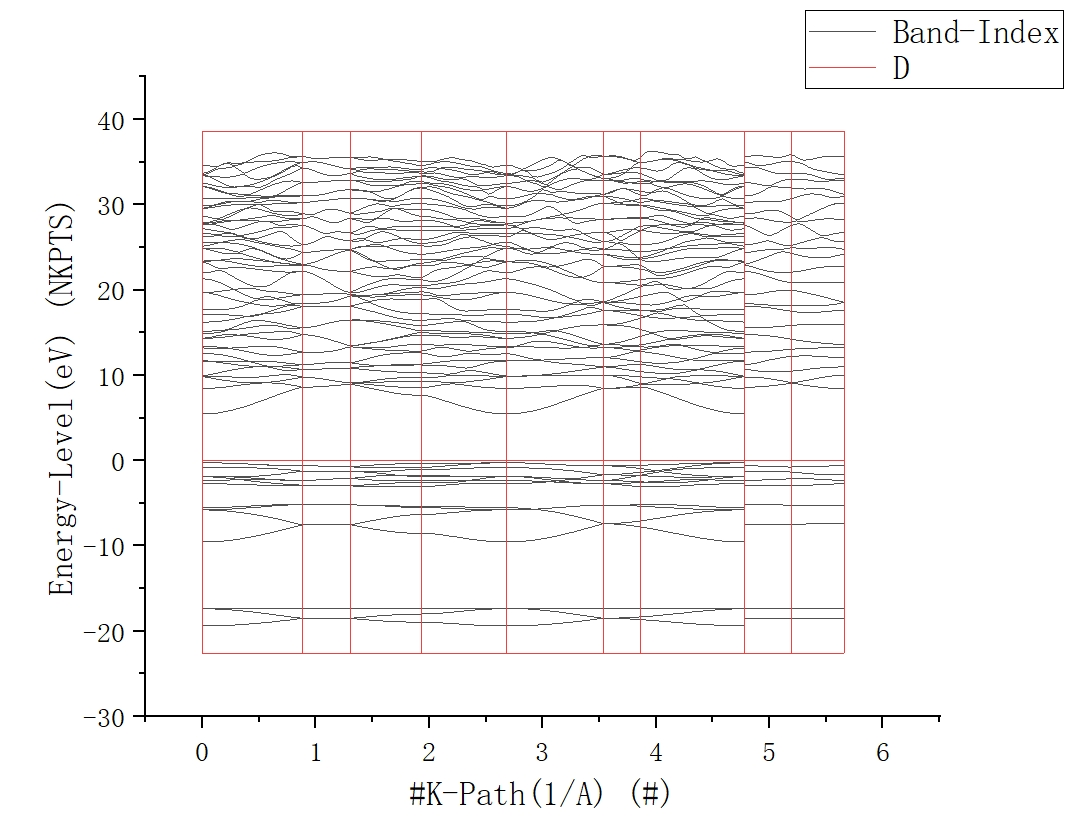
\includegraphics[width=1\linewidth]{VASP计算/能带计算/能带绘图与后处理/fig/Origin生成能带.png}
    \caption{Origin生成的能带图}
    \label{fig:能带绘图与后处理-Origin生成的能带图}
\end{figure}

调整线型与坐标范围,并在下方添加高对称点标签(可以借助于vaspkit生成的\code{KLABELS}文件,其中包含所有高对称点坐标所对应的x轴坐标)

\begin{attention}
    一般来说,默认生成的能带图都会如图\ref{fig:能带绘图与后处理-Origin生成的能带图}所示包含较多的能带。但在实际研究中,我们往往仅关心费米能级附近(即0点附近)的情况。此时除了可以使用Origin调整坐标轴范围的方法,也可以在使用VASP计算自洽和能带的时候使用\code{NBANDS}参数,设置\emph{需要显示的能带数量}。

    在使用vaspkit自动生成能带图时,则需要对这一参数进行设置。
\end{attention}

处理后得到的能带图如图\ref{fig:能带绘图与后处理-SiO2能带图}所示\footnote{绘图配色可以根据自己喜好选择。}

\begin{figure}
    \centering
    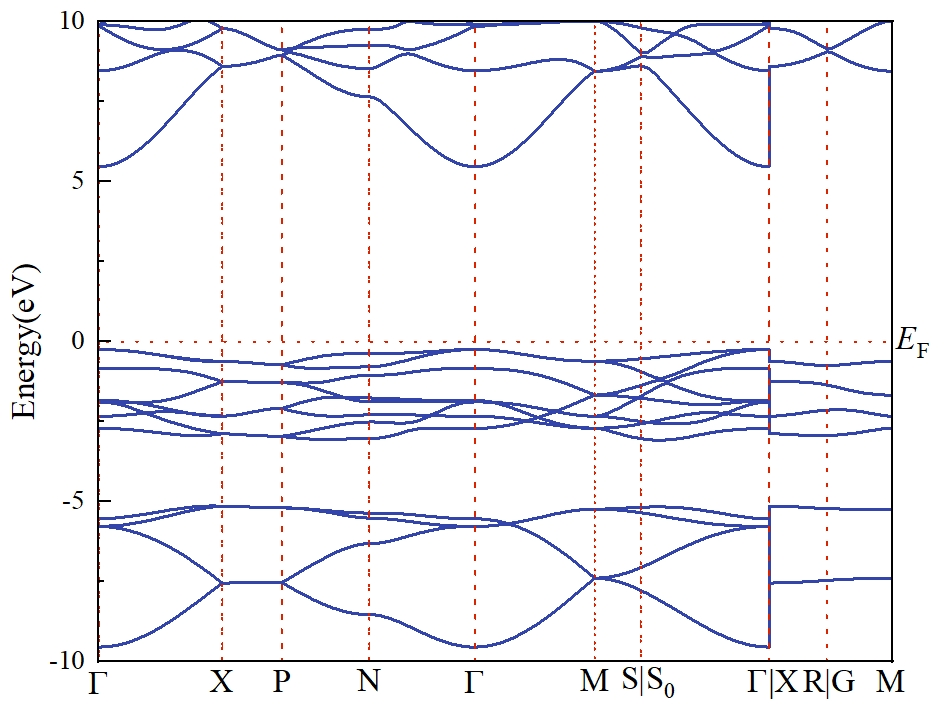
\includegraphics[width=1\linewidth]{VASP计算/能带计算/能带绘图与后处理/fig/SiO2能带图.png}
    \caption{\ch{SiO2}能带图}
    \label{fig:能带绘图与后处理-SiO2能带图}
\end{figure}

\subsection{使用vaspkit自动生成能带图}\label{subsec:能带绘图与后处理-使用vaspkit自动生成能带图}

自1.2.5版本之后,vaspkit更新了自动绘图的功能。利用这一功能,可以不将数据下载至本地后使用Origin绘图,而是直接在Linux操作系统中得到能带图像。

使用vaspkit自动绘图的过程是比较简单的,但我们需要提前对vaspkit做一些配置上的设置。

\subsubsection{vaspkit配置过程}

\begin{attention}
    请首先检查你所使用的vaspkit是否为1.2.5或更新版本。你可以直接使用\code{vaspkit}命令,在菜单栏上方,可以查看所使用的软件版本。

    同时,你还应当确认你的系统上已经配置了Python相关环境,以及绘图所必须的matplotlib包。通常,使用Anaconda可以“一次性”完成Python所需要的所有配置。确认是否安装Anaconda的一个方法是使用命令\code{conda --version},若输出版本号,则表明已经配置了Anaconda\footnote{在有些服务器上,可能需要其他设置引入Anaconda模块。例如,在我所在课题组的服务器上,使用之前需要调用\code{module load anaconda3}导入相关模块。}。

    如果存在没有的命令或模块,可能需要重新安装。详细安装过程请查阅对应软件官网\footnote{VASPKIT官网:https://vaspkit.com/}\footnote{Anaconda官网:https://www.anaconda.com/}的说明。
\end{attention}

假设你的系统已经确认可以配置,在开始之前还需要做如下操作:

\begin{enumerate}
    \item 使用\code{which python3}查看\emph{python3所在目录}。你需要记住这一路径,将其首先复制到本地的记事本或其他地方是一个好方法;
    \item 使用\code{which vaspkit}查看\emph{vaspkit所在目录},并使用\code{cd}命令进入这一目录(通常只需要进入到版本号所在目录即可,例如,在我所在课题组当中,目录为\code{/opt/pub/softwares/VASPKIT/1.5.1});
    \item 在这一目录下,找到\code{how\_to\_set\_environment\_variables}文件,并将其中从\code{\#BEGIN\_CUSTOMIZE\_PLOT}到\code{\#END\_CUSTOMIZE\_PLOT}之间的所有内容(包括这两行)复制到某个地方,以便稍后使用;
    \item 回到所在家目录,新建一个\code{.vaspkit}文件,并在其中创建如下两行:
    \begin{lstlisting}[caption=.vaspkit]
PYTHON_BIN    /opt/pub/toolkits/anaconda3/bin/python3
AUTO_PLOT     .TRUE.
    \end{lstlisting}
    其中,\code{PYTHON\_BIN}后面对应的是之前所复制的python3所在目录。然后,在文件下方将所复制的\code{\#BEGIN\_CUSTOMIZE\_PLOT}到\code{\#END\_CUSTOMIZE\_PLOT}之间的所有内容粘贴至后面。
\end{enumerate}

\subsubsection{使用vaspkit绘图}

在使用vaspkit绘图前,应当首先保证你已经导入了相应模块(如Anaconda等)。与正常使用vaspkit导出能带图类似,在使用\code{vaspkit-211}导出时,会询问导出图片是仅导出能带图,还是能带图加态密度。我们在这里选择仅绘制能带图(1),得到如图所示的图像。

\begin{figure}
    \centering
    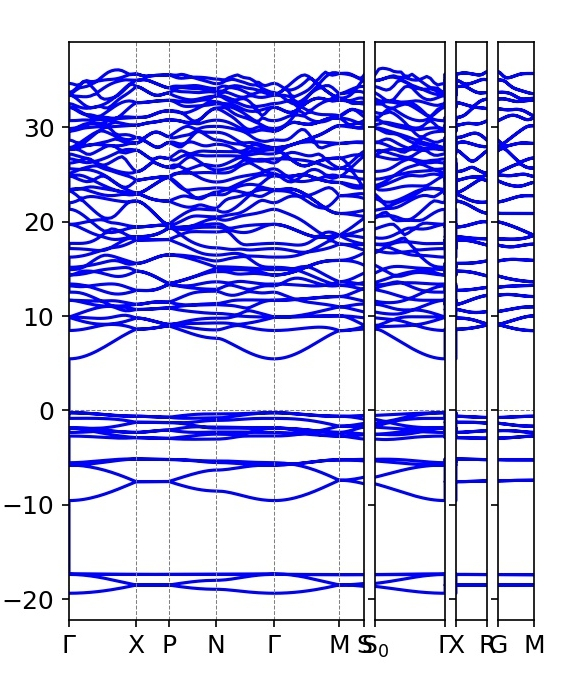
\includegraphics[width=1\linewidth]{VASP计算/能带计算/能带绘图与后处理/fig/vaspkit自动生成能带图.png}
    \caption{使用vaspkit生成能带图}
    \label{fig:使用vaspkit生成能带图}
\end{figure}

\begin{extend}
    正如你所见那样,使用vaspkit默认生成的能带图是很大的能量范围,且不能对其进行调整。一个简单的方法是在计算时使用\keyword{EMIN}和\keyword{EMAX}参数设置能量区间。
\end{extend}

\subsection{如何计算带隙}\label{subsec:能带绘图与后处理-如何计算带隙}

有时,我们可能不是强制要求需要得到能带图,而仅仅关注结构的带隙性质(如带隙大小,类型等)。此时,可以直接使用在绘图过程中生成的\code{BAND\_GAP}文件(使用\code{vaspkit-211}生成)。以\ch{SiO2}为例,文件内容为:

\begin{lstlisting}[caption=BAND\_GAP]
Band Character:    Direct
Band Gap (eV):    5.7105
Eigenvalue of VBM (eV):   -0.6699
Eigenvalue of CBM (eV):    5.0407
Fermi Energy (eV):   -0.4270
HOMO & LUMO Bands:        16        17
Location of VBM: -0.000000  0.000000  0.000000
Location of CBM: -0.000000  0.000000  0.000000
\end{lstlisting}

其中,\code{Band Character}表明带隙类型是直接带隙(Direct)或间接带隙(Inderect);\code{Band Gap}表明所计算结构的带隙大小,在本例中为5.71 eV。除此之外,这一文件还提供了如HOMO(最高占据分子轨道)和LUMO(最低未占据分子轨道)所对应的能带条数,以及VBM(价带顶)和CBM(导带底)所对应的K点坐标。

\begin{attention}
    如果你关注过最开始Materials Project所记录的数据,可能会发现,数据库内所给的带隙约为5.8 eV。而我们所计算得到的比实际带隙小了约0.1 eV。正如\ref{sec:VASP计算能带过程}开始所说的那样,这一误差是由于PBE泛函所导致的,而这是PBE泛函的固有缺陷。在一些需要精确计算的情况下,我们可能希望计算HSE能带而不是PBE能带。
\end{attention}


% \subsection{错误处理}\label{subsec:节标题-错误处理}
% % 请在本节列出可能遇见的错误与解决方法

% \subsubsection{错误1}

% \subsubsection{错误2}

% \subsubsection{错误3}
\chapter{声子谱计算}\label{chap:声子谱计算}
\minitoc
\section{什么是声子、声子谱} \label{sec:什么是声子、声子谱}

\sectionAuthor{Isay K.}

\begin{Abstract}
    \item 声子
    \item 声子谱
\end{Abstract}

\subsection{声子}\label{subsec:什么是声子、声子谱-声子}

声子(Phonon),即“晶格振动的简正模能量量子”,是晶体中\emph{原子振动}的量子化描述。

在固体物理学中,声子是晶格振动的准粒子,其携带能量和动量,并且可以像粒子一样进行相互作用。

声子是\emph{简谐近似}下的产物,如果振动太剧烈,超过小振动的范围,那么晶格振动就要用非简谐振动理论描述。

声子并不是一个真正的粒子,声子可以产生和湮灭,有相互作用的声子数不守恒,声子动量的守恒律也不同于一般的粒子,并且声子不能脱离固体存在。声子只是格波激发的量子,在多体理论中称为集体振荡的元激发或准粒子。

声子的化学势为零,属于\emph{玻色子},服从玻色-爱因斯坦统计。声子本身并不具有物理动量,但是携带有准动量,并具有能量,它的能量等于$\hbar\omega_q$。

声子可以分为以下两类:
\begin{itemize}
    \item 声学支:与晶格的纵向和横向振动相关,类似于声波,表示原胞的整体振动。
    \item 光学支:与晶格的非均匀振动相关,通常与电荷的重新分布有关,表示原胞内原子间的相互振动。
\end{itemize}

如果一个材料的原胞中有$N$个原子,那么声子谱就会有$3N$支,其中3条声学支,$3N-3$条光学支。

\subsection{声子谱}\label{subsec:什么是声子、声子谱-声子谱}

声子谱,也称为声子色散关系,是描述声子能量与动量之间关系的图表。

声子谱通常在第一布里渊区内绘制,因为其包含了所有可能的声子模式。

通常,使用声子谱研究体系的动力学稳定性,使用分子动力学研究体系的热力学稳定性。

声子谱的其他物理意义:
\begin{itemize}
    \item 电子-声子耦合:在半导体和超导体中,电子-声子耦合相互作用对材料的电子性质至关重要;
    \item 声子散射:在金属和半导体中,声子散射是影响电子迁移率的关键因素;
    \item 热容:声子谱可以解释材料在不同温度下的热容行为
    \item ...
\end{itemize}

\section{计算方法简介}\label{sec:计算方法简介}

\sectionAuthor{Isay K.}

\begin{Abstract}
    \item 密度泛函微扰理论(DFPT)
    \item 有限位移法(Finite Displacement Method)
    \item 适用情境比较
\end{Abstract}


\subsection{密度泛函微扰理论(DFPT)}\label{subsec:计算方法简介-密度泛函微扰理论(DFPT)}

DFPT是一种基于第一性原理的方法,它直接从周期性边界条件的Kohn-Sham波函数计算出声子谱。在DFPT中,通过计算原子间相互作用的微扰来得到力常数矩阵,这是描述晶格动力学性质的关键量。

\begin{extend}
    1987年,Baroni、Giannozzi和Testa提出了一种新的晶格动力学性质计算方法--微扰密度泛函方法(Density Function Perturbation Theory)。DFPT通过计算系统能量对外场微扰的响应来求出晶格动力学性质。该方法最大的优势在于它不限定微扰的波矢与原胞边界(super size)正交,不需要超原胞也可以对任意波矢求解。因此可以应用到复杂材料性质的计算上。此外,能量对外场微扰的响应不仅可以推导出声子的晶体性质,还能求出弹性系数、声子展宽、拉曼散射截面等性质,这种方法本身就能算出Born effective charge dielectric constant,可以很好的预言LO-TO splitting甚至Kohn anomalies。这些优势使得DFPT一经提出就被广泛应用到了半导体、金属和合金、超导体等材料的计算上。比较常用的程序是pwscf和abinit,castep等采用的是一种linear response theory 的方法(或者称为  density perturbation functional theory,DFPT),直接计算出原子的移动而导致  的势场变化,再进一步构造出动力学矩阵。
\end{extend}

\subsection{有限位移法(Finite Displacement Method)}\label{sec:计算方法简介-有限位移法(Finite Displacement Method)}

有限位移法通过在超原胞中引入原子的有限位移来模拟晶格振动。这种方法基于位移-响应理论,通过计算原子位移后系统的受力来构造动力学矩阵

\begin{extend}
    直接法,或称frozen-phonon方法,是通过在优化后的平衡结构中引入原子位移,计算作用在原子上的Hellmann-Feynman力,进而由动力学矩阵算出声子色散曲线。用该方法计算声子色散曲线最早开始于80年代初,由于计算简便,不需要特别编写的计算程序,很多小组都采用直接法计算材料性质。直接法的缺陷在于它要求声子波矢与原胞边界(super size)正交,或者原胞足够大使得Hellmann-Feynman力在原胞外可以忽略不计。这使得对于复杂系统,如对称性高的晶体、合金、超晶格等材料需要采用超原胞。超原胞的采用使计算量急剧增加,极大的限制了该方法的使用。这种方法不能很好的预言LO-TO splitting,只有在计算了Born effective charge和dielectric constant之后,进一步考虑了non-analyticity term,才能计算出;但Direct Method本身并不能给出Born effective charge和dielectric constant,所以这也是它的一个缺陷。
\end{extend}

\subsection{适用情境比较}\label{subsec:计算方法简介-适用情境比较}

DFPT适用情境:
\begin{itemize}
    \item 需要高精度声子谱的系统,尤其是小到中等大小的晶胞;
    \item 研究者希望避免有限位移法可能引入的系统误差时。
\end{itemize}
\begin{attention}
    DFPT方法计算成本较高,尤其对于大晶胞或高对称点附近的计算。
\end{attention}

有限声子法适用情境:
\begin{itemize}
    \item 当计算资源有限或需要对多种材料进行筛选时;
    \item 对于大晶胞材料的初步声子谱分析。
\end{itemize}

总得来说,对于较重的任务,DFPT方法可能会造成内存溢出,且DFPT方法由于其特性而无法进行并行计算,而有限声子法可以并行。对于较小的体系,可以根据需要和组内资源选择方法。

\begin{extend}
    建议优先使用有限位移法。

    一些教程中有时候将有限位移法又称为冷冻声子法或直接法。
    但笔者并没有找到更官方的资料说明有限位移法和冷冻声子法是同一种方法,谨奉上PHONOPY官网供读者自行分辨:https://phonopy.github.io/phonopy/index.html
\end{extend}

参考:
http://muchong.com/html/200802/723527.html
\section{计算软件PHONOPY}\label{sec:计算软件PHONOPY}

\sectionAuthor{Isay K.}

在本节,你将要学到:
\begin{Abstract}
    \item 开始安装之前
    \item PHONOPY快速安装
    \item PHONOPY使用方法
\end{Abstract}

\subsection{开始安装之前}\label{subsec:计算软件PHONOPY-开始安装之前}

由于本教程面向的群体是计算小白(包括笔者也是通过本教程记录一下自己掉的坑),所以在开始安装软件之前,我们强烈建议先咨询组内老师或师兄师姐:服务器上是否已经配置了相应的软件?

\begin{extend}
    当然也可以使用 module avail 命令自己检查系统内已安装的软件,如果没有找到的话再咨询更有自主性哦。
    \begin{figure}
        \centering
        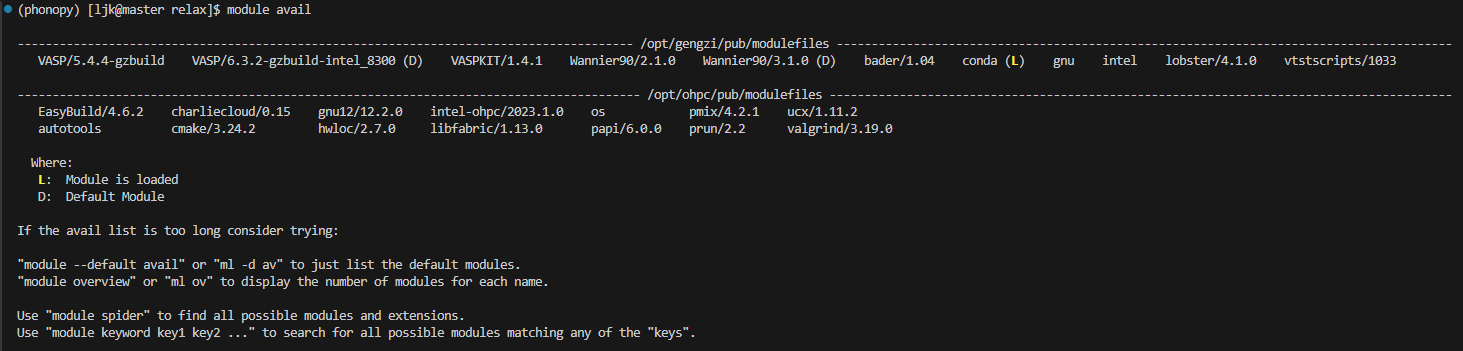
\includegraphics[width=1\linewidth]{module-check.png}
        \caption{检查是否含有所需软件}
        \label{fig:检查软件}
    \end{figure}
\end{extend}

通常情况下,组内服务器的\emph{根目录}下已经配置了相应的软件,这个时候再在自己的\emph{用户目录}下进行配置的话,一方面在使用过程中可能会出现命令的冲突,另一方面也是一种时间、精力和资源的浪费。

如果组内确实并没有安装,或者你是传说中的开山大弟子,又或者是自学,请放心进入\ref{subsec:计算软件PHONOPY-PHONOPY快速安装}小节。

\subsection{PHONOPY快速安装}\label{subsec:计算软件PHONOPY-PHONOPY快速安装}

% 聪明的小朋友从图\ref{fig:检查软件}中其实已经可以看出端倪,图中并没有PHONOPY模块。

% 这是因为使用传统的安装方式较为麻烦,而且PHONOPY新版本需要\emph{python>=3.7.0},需要自行安装python等多个模块。因此我们借助一个神器——Anaconda——进行PHONOPY的安装。

% 写着写着突然想起
% \subsubsection{Anaconda安装}

% Anaconda的官网:
% https://www.continuum.io/downloads/

% 官网需要翻墙,可以使用清华的镜像网站:
% https://mirrors.tuna.tsinghua.edu.cn/anaconda/archive/

% \begin{figure}
%     \centering
%     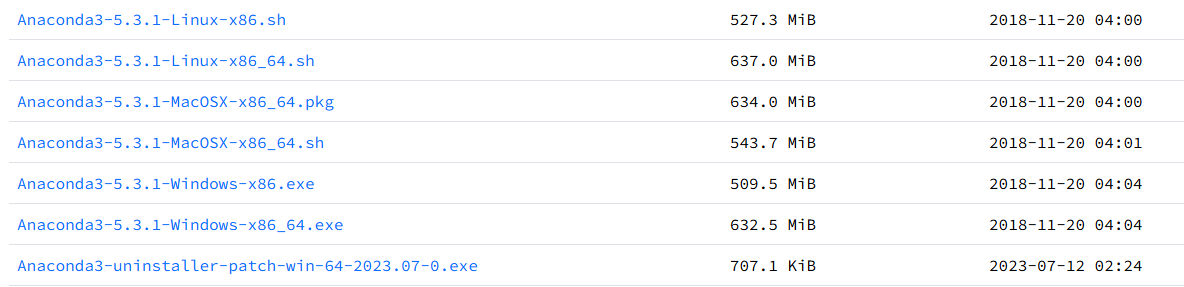
\includegraphics[width=1\linewidth]{mirror.png}
%     \caption{镜像网站}
%     \label{fig:镜像网站}
% \end{figure}

% 图\ref{fig:镜像网站}中,x86是32位的,x86\_64是64位的,根据服务器的系统型号下载即可。

% 将下载好的.sh文件放在服务器的根目录下,进入该目录

参考:
https://blog.csdn.net/qq\_41866202/article/details/124407208?spm=1001.2101.3001.6661.1\&utm\_medium=distribute.pc\_relevant\_t0.none-task-blog-2\%7Edefault\%7EBlogCommendFromBaidu\%7ECtr-1-124407208-blog-139391379.235\%5Ev43\%5Epc\_blog\_bottom\_relevance\_base9\&depth\_1-utm\_source=distribute.pc\_relevant\_t0.none-task-blog-2\%7Edefault\%7EBlogCommendFromBaidu\%7ECtr-1-124407208-blog-139391379.235\%5Ev43\%5Epc\_blog\_bottom\_relevance\_base9\&utm\_relevant\_index=1

\subsection{PHONOPY使用方法}\label{subsec:计算软件PHONOPY-PHONOPY使用方法}

\subsubsection{加载PHONOPY环境}
\begin{enumerate}
    \item 加载Anaconda应用:\code{module load conda}
    \item 激活PHONOPY环境:\code{conda activate PHONOPY}
\end{enumerate}

\subsubsection{命令详解}

进入下面的官网之后点击Command options即可看到所有功能。

https://phonopy.github.io/phonopy/index.html 

\begin{attention}
 在进行扩胞时的标准是:扩胞后的原子达到80\ttilde100个,每个晶轴方向大于10,不然得到的声子谱中很容易出现虚频。
\end{attention}
\section{具体计算步骤}\label{sec:具体计算步骤}

\sectionAuthor{Isay K.}

\begin{Abstract}
    \item 计算声子谱前的结构优化
    \item DFPT方法计算声子谱
    \item 有限位移法计算声子谱
\end{Abstract}

\subsection{计算声子谱前的结构优化}\label{sec:具体计算步骤-计算声子谱前的结构优化}

\begin{attention}
  在计算声子时需要先对原胞结构做高精度的结构优化,不然得到的声子谱中很容易出现虚频。  
\end{attention}

我们以$TiTe_2$为例,以下是高精度优化的具体参数。

\begin{lstlisting}[caption=INCAR]
Global Parameters
ISTART =  1            (Read existing wavefunction, if there)
ISPIN  =  1            (Non-Spin polarised DFT)
LREAL  = .FALSE.       (Projection operators: automatic)
ENCUT  =  380        (Cut-off energy for plane wave basis set, in eV)

LWAVE  = .FALSE.        (Write WAVECAR or not)
LCHARG = .FALSE.        (Write CHGCAR or not)
ADDGRID= .TRUE.        (Increase grid, helps GGA convergence)
LASPH  = .TRUE.        (Give more accurate total energies and band structure calculations)
PREC   = Accurate      (Accurate strictly avoids any aliasing or wrap around errors)
NCORE = 8 
ISYM = 0

Lattice Relaxation
NSW    =  300          (number of ionic steps)
ISMEAR =  0            (gaussian smearing method )
SIGMA  =  0.03         (please check the width of the smearing)
IBRION =  2            (Algorithm: 0-MD, 1-Quasi-New, 2-CG)
ISIF   =  3            (optimize atomic coordinates and lattice parameters)
IOPTCELL = 1 0 0 1 1 0 0 0 0
EDIFF = 1E-08
EDIFFG = -1E-03      (Ionic convergence, eV/A)
\end{lstlisting}

为了保证优化精度足够高,其中需要注意的是:
\begin{enumerate}
    \item EDIFF表示电子收敛标准,至少要取1E-06,体系小的话尽量取1E-08;
    \item EDIFFG取负值时表示力收敛标准,取1E-03;
    \item ADDGRID表示是否添加额外网格提高精度,设定为.TRUE.;
    \item PREC表示“精度”模式,设定为Accurate(准确);
    \item NSW表示电子优化步数,取300防止计算中断;
    \item ENCUT可以自行做测试,详见VASP计算-结构优化章节(先别去找,我没写);
\end{enumerate}

另外,其中ISIF=3表示既优化晶格又优化原子坐标,配合IOPTCELL可以实现晶轴的单独固定,以达到计算二维材料的目的,详见VASP计算-结构优化章节(也还没写)。

下面的其他输入文件没有需要特别说明的,如有疑问请参考VASP计算-结构优化章节(哈哈,又是这)或参考VASP官网:https://www.vasp.at/wiki/index.php/The\_VASP\_Manual

\begin{lstlisting}[caption=KPOINTS]
A
0
Gamma
24   24   1
0.0  0.0  0.0
\end{lstlisting}

\begin{lstlisting}[caption=POSCAR]
 TiTe2-1m1                               
    1.00000000000000     
      3.7458432095936396   -0.0000184453725456    0.0000000000000000
     -1.8729216047968198    3.2439861579338527    0.0000000000000000
      0.0000000000000000    0.0000000000000000   18.0000000000000000
    Ti   Te
      1     2
 Direct
   0.0000000000000000  0.0000000000000000  0.5127400160000022
   0.6666666132020026  0.3333334158033583  0.6098496477195335
   0.3333334157979960  0.6666666131966403  0.4156403382804701
  
   0.00000000E+00  0.00000000E+00  0.00000000E+00
   0.00000000E+00  0.00000000E+00  0.00000000E+00
   0.00000000E+00  0.00000000E+00  0.00000000E+00
\end{lstlisting}

\begin{lstlisting}[caption=POTCAR]
    (结构优化章节)
\end{lstlisting}

提交任务进行计算,得到CONTCAR为优化后的更合理的结构,作为后续声子计算的初始晶胞。
(后续小节中提到“初始晶胞”均指优化后得到的晶胞,为避免歧义在此说明。)

 
\subsection{DFPT方法计算声子谱}\label{sec:具体计算步骤-DFPT方法计算声子谱}

1.\code{mkdir method\_DFPT}

新建文件夹。

2.\code{cp relax/CONTCAR method\_DFPT/POSCAR}

将上一步高精度结构优化得到的CONTCAR复制进文件夹内,并重命名为POSCAR。

3.\code{cd method\_DFPT}

进入新文件夹。

4.\code{module load conda}
\code{conda activate phonopy}

加载conda模块,并激活phonopy环境,详情可参考\ref{sec:计算软件PHONOPY-PHONOPY使用方法}

5.\code{phonopy -d --dim="6 6 1"}

使用PHONOPY进行6×6的扩胞。

此时会产生数个名为POSCAR-0?的位移文件,以及名为SPOSCAR的扩胞后的结构。

DFPT方法使用的是SPOSCAR,而有限位移法使用的是这些位移文件。

\begin{attention}
   笔者研究的是2D结构,仅对两个方向进行扩胞,读者可根据需要自行调整。
   扩胞的标准是扩胞后达到80~100个原子,且晶轴长度大于10埃,不然得到的声子谱中很容易出现虚频。
\end{attention}

6.\code{mkdir vasp-calculations}

新建文件夹用于后续计算。

\begin{extend}
  此处根据个人习惯不同,也可以不新建文件夹。将POSCAR重命名为POSCAR-unit,将第5步新产生的SPOSCAR重命名为POSCAR,直接在当前文件夹中进行计算。
\end{extend}

7.\code{cp SPOSCAR vasp-calculations/POSCAR}

将第5步新产生的SPOSCAR复制进文件夹,并重命名为POSCAR。

8.准备其它基本文件:

\begin{lstlisting}[caption=INCAR]
SYSTEM = TiTe2
#ISIF = 3
NSW = 1
IBRION = 8

LWAVE = F
LCHARG = F

ENCUT = 380
EDIFF = 1E-8
EDIFFG =-1E-3
ISMEAR = 0

LREAL = F
SIGMA = 0.03

PREC = A
ADDGRID = .TRUE.
\end{lstlisting}

\begin{lstlisting}[caption=KPOINTS]
  A
  0
  Gamma
  3   3   1
  0.0  0.0  0.0
\end{lstlisting}

\begin{attention}
 因为该计算使用的是扩胞之后的结构,所以K点没有必要取太大。
\end{attention}

\begin{lstlisting}[caption=POTCAR]
  老方法
\end{lstlisting}


9.\code{sbatch sub.vasp}

提交任务进行计算。

10.\code{cd ..}

返回method\_DFPT文件夹。

11.\code{cp vasp-calculations/vasprun.xml .}

将vasprun.xml复制到当前文件夹。

12.\code{phonopy --fc vasprun.xml}

使用phonopy读取vasprun.xml生成力常数文件FORCE\_CONSTANTS。

13.\code{vi band.conf}

编辑band.conf文件:
\begin{lstlisting}[caption=band.conf]
ATOM_NAME =Ti Te
DIM = 6 6 1
BAND =0 0 0  0.5 0 0  0.33333 0.33333 0   0 0 0
BAND_POINTS = 101
FORCE_CONSTANTS = READ
\end{lstlisting}

\begin{enumerate}
    \item DIM根据体系的扩胞大小设置,如扩胞扩到332,就设置成332。
    \item BAND和能带的取点是一样的,也可以用vaspkit生成。
    \item FORCE\_CONSTANTS一定设置成READ。
    \item 更多设置可以看PHONOPY官网。
\end{enumerate}

14.\code{phonopy -p -s band.conf}

使用phonopy读取band.conf文件,作图并保存。

15.\code{phonopy-bandplot --gnuplot > phonon.out}

将数据导出方便后续用Origin等软件重新绘图。

\begin{extend}
  旧版本的phonopy的导出命令为:\code{bandplot  --gnuplot> phonon.out}
\end{extend}

\subsection{有限位移法计算声子谱}\label{sec:具体计算步骤-有限位移法计算声子谱}

1.\code{mkdir method\_yxwy}

2.\code{cp relax/CONTCAR method\_yxwy/POSCAR}

3.\code{cd method\_yxwy}

4.\code{phonopy -d --dim="6 6 1"}

前四步和DFPT法完全相同。

5.\code{for i in {01..12}; do mkdir \$i; cp POSCAR-0\$i \$i/POSCAR;done}

假如第四步产生了12个位移文件,使用for循环生成12个文件夹,并将对应的位移POSCAR移入文件夹重命名为POSCAR。

6.准备其它基本文件:

\begin{lstlisting}[caption=INCAR]
ADDGRID = .TRUE.
PREC = Accurate
IBRION = -1
ENCUT = 380
EDIFF = 1E-8
EDIFFG = -1E-3

ISMEAR = 0
SIGMA = 0.03

IALGO = 38

LREAL = .FALSE.
LWAVE = .FALSE.
LCHARG = .FALSE.

NCORE = 4
\end{lstlisting}

\begin{attention}
 有限位移法的单个计算实际上就是高精度的静态自洽。
\end{attention}

\begin{lstlisting}[caption=KPOINTS]
Automatic mesh
0
Gamma
3 3 1
0 0 0
\end{lstlisting}

\begin{attention}
 同DFPT法一样,有限位移法使用的也是扩胞之后的结构,所以K点没有必要取太大。
\end{attention}

7.\code{for i in {01..12}; do cp INCAR KPOINTS POTCAR sub.vasp \$i; cd \$i; sbatch sub.vasp; cd \$OLDPWD;done}

将基本文件复制进各个小文件夹中并进行计算。

8.\code{phonopy -f {01..12}/vasprun.xml}

计算全部结束后,使用phonopy读取全部的计算文件夹中的vasprun.xml,生成FORCE\_SETS文件。

9.\code{vi band.conf}

\begin{lstlisting}[caption=band.conf]
  ATOM_NAME =Ti Te
  DIM = 6 6 1
  BAND =0 0 0  0.5 0 0  0.33333 0.33333 0   0 0 0
  BAND_POINTS = 101
  FORCE_SETS = READ
\end{lstlisting}

与DFPT方法唯一不同的部分在于将FORCE\_CONSTANTS=READ改成FORCE\_SETS=READ。

10.\code{phonopy -p -s band.conf}

使用phonopy读取band.conf文件,作图并保存。

11.\code{phonopy-bandplot --gnuplot > phonon.out}

将数据导出方便后续用Origin等软件重新绘图。

\section{声子谱分析}\label{sec:声子谱分析}

\sectionAuthor{Isay K.}

我还不太会,等我学学。

http://pubs.acs.org/doi/abs/10.1021/acs.jpcc.5b04669
\section{错误处理}\label{sec:错误处理}
vasprun.xml没有必要信息

    \part{Python与机器学习}

    \include{Python与机器学习/Python_main}

    \backmatter

    \printindex

    \bibliography{reference}

\end{document}